\documentclass[12pt,a4paper,oneside]{report}

% ---------------------------------------------------------------- Encodage & langue
\usepackage[utf8]{inputenc}
\usepackage[T1]{fontenc}
\usepackage[english,french]{babel}
\addto\captionsfrench{\renewcommand{\tablename}{Tableau}\renewcommand{\listfigurename}{Liste des figures}\renewcommand{\listtablename}{Liste des tableaux}}
\usepackage{lmodern}
\usepackage{microtype}

% ---------------------------------------------------------------- Mise en page
\usepackage[a4paper,top=2.5cm,bottom=2.5cm,left=2.5cm,right=2.5cm,headheight=15pt]{geometry}
\usepackage{setspace}
\onehalfspacing
\usepackage{fancyhdr}
\usepackage{titlesec}
\usepackage{enumitem}
\setlist{itemsep=2pt,topsep=4pt}

% ---------------------------------------------------------------- Figures, tableaux
\usepackage{graphicx}
\graphicspath{{images/}}
\usepackage{float}
\usepackage[font=small,labelfont=bf]{caption}
\usepackage{booktabs}
\usepackage{tabularx}
\usepackage{longtable}
\usepackage{multirow}
\usepackage{array}
\usepackage[table]{xcolor}
\usepackage{tikz}
\usetikzlibrary{arrows.meta,positioning,shapes.geometric,shapes.misc,fit,backgrounds,calc,shadows}
\usepackage{listings}
\renewcommand{\tabularxcolumn}[1]{>{\raggedright\arraybackslash}p{#1}}

% ---------------------------------------------------------------- Liens & abréviations
\usepackage{xurl}
\usepackage[hidelinks,unicode]{hyperref}
\usepackage[acronym,nonumberlist,nopostdot,toc]{glossaries}

% ---------------------------------------------------------------- Couleurs du rapport
\definecolor{bleu}{HTML}{1F4E79}
\definecolor{bleuclair}{HTML}{DCE6F2}
\definecolor{vert}{HTML}{2E7D32}
\definecolor{vertclair}{HTML}{E8F5E9}
\definecolor{orange}{HTML}{E65100}
\definecolor{orangeclair}{HTML}{FFF3E0}
\definecolor{rouge}{HTML}{B71C1C}
\definecolor{rougeclair}{HTML}{FFEBEE}
\definecolor{gris}{HTML}{555555}
\definecolor{grisclair}{HTML}{F2F2F2}

% Marqueur pour les éléments à compléter avec les vrais résultats
\newcommand{\AFAIRE}[1]{\textcolor{red}{\textbf{[À compléter : #1]}}}

% ---------------------------------------------------------------- Titres
\titleformat{\chapter}[display]
  {\normalfont\bfseries\color{bleu}}
  {\LARGE\chaptertitlename\ \thechapter}{8pt}{\Huge}
\titlespacing*{\chapter}{0pt}{0pt}{30pt}
\titleformat{\section}{\normalfont\Large\bfseries\color{bleu}}{\thesection}{1em}{}
\titleformat{\subsection}{\normalfont\large\bfseries}{\thesubsection}{1em}{}

% ---------------------------------------------------------------- En-têtes
\pagestyle{fancy}
\fancyhf{}
\renewcommand{\chaptermark}[1]{\markboth{\chaptername\ \thechapter.\ #1}{}}
\fancyhead[L]{\small\textsc{\nouppercase{\leftmark}}}
\fancyhead[R]{\small\thepage}
\renewcommand{\headrulewidth}{0.4pt}
\fancypagestyle{plain}{\fancyhf{}\fancyfoot[C]{\small\thepage}\renewcommand{\headrulewidth}{0pt}}

% Chapitre non numéroté : titre, entrée au sommaire et en-tête corrects
\newcommand{\chapitresansnumero}[1]{%
  \chapter*{#1}\addcontentsline{toc}{chapter}{#1}\markboth{#1}{#1}}

% ---------------------------------------------------------------- Code
\lstset{basicstyle=\ttfamily\small,frame=single,backgroundcolor=\color{grisclair},
  numbers=left,numberstyle=\tiny\color{gris},breaklines=true,columns=fullflexible,
  keepspaces=true,showstringspaces=false}
\renewcommand{\lstlistingname}{Code}

% ---------------------------------------------------------------- Styles TikZ communs
\tikzset{
  boite/.style={draw=bleu,rounded corners=3pt,fill=bleuclair,align=center,
                font=\small,inner sep=5pt,minimum height=0.9cm},
  fleche/.style={-{Stealth[length=2.5mm]},thick,color=gris},
}

\makeglossaries
\newacronym{ai}{IA}{Intelligence Artificielle}
\newacronym{api}{API}{Application Programming Interface}
\newacronym{bpl}{BPL}{Bone Phosphate of Lime}
\newacronym{dt}{DT}{Digital Twin (jumeau numérique)}
\newacronym{dtc}{DTC}{Digital Twin Consortium}
\newacronym{epcm}{EPCM}{Engineering, Procurement and Construction Management}
\newacronym{feed}{FEED}{Front-End Engineering Design}
\newacronym{gmao}{GMAO}{Gestion de Maintenance Assistée par Ordinateur}
\newacronym{hmi}{IHM}{Interface Homme-Machine}
\newacronym{iiot}{IIoT}{Industrial Internet of Things}
\newacronym{iot}{IoT}{Internet of Things}
\newacronym{isa}{ISA}{International Society of Automation}
\newacronym{jwt}{JWT}{JSON Web Token}
\newacronym{kpi}{KPI}{Key Performance Indicator}
\newacronym{llm}{LLM}{Large Language Model}
\newacronym{mae}{MAE}{Mean Absolute Error}
\newacronym{ml}{ML}{Machine Learning}
\newacronym{mqtt}{MQTT}{Message Queuing Telemetry Transport}
\newacronym{opcua}{OPC UA}{Open Platform Communications Unified Architecture}
\newacronym{ot}{OT}{Operational Technology}
\newacronym{p80}{P80}{Taille de maille laissant passer 80\,\% de la masse du produit}
\newacronym{pfa}{PFA}{Projet de Fin d'Année}
\newacronym{plc}{PLC}{Programmable Logic Controller (automate programmable)}
\newacronym{poc}{PoC}{Proof of Concept (preuve de concept)}
\newacronym{rag}{RAG}{Retrieval-Augmented Generation}
\newacronym{rmse}{RMSE}{Root Mean Square Error}
\newacronym{scada}{SCADA}{Supervisory Control And Data Acquisition}
\newacronym{spa}{SPA}{Single Page Application}
\newacronym{uml}{UML}{Unified Modeling Language}


\begin{document}

\begin{titlepage}
\begin{center}
\begin{minipage}{0.22\textwidth}
\includegraphics[width=0.75\linewidth]{logo_ensem}\end{minipage}\hfill
\begin{minipage}{0.5\textwidth}\centering\small\bfseries
Université Hassan II de Casablanca\\[2pt]
École Nationale Supérieure d'Électricité et de Mécanique
\end{minipage}\hfill
\begin{minipage}{0.22\textwidth}\raggedleft
\includegraphics[width=0.85\linewidth]{logo_uh2c}\end{minipage}

\vspace{0.4cm}
{\color{bleu}\rule{\linewidth}{1pt}}

\vspace{0.8cm}
{\large Département Génie Électrique}\\[4pt]
{\large Filière : DPI -- 3\textsuperscript{e} année}

\vspace{1.2cm}
{\Large\bfseries RAPPORT DE PROJET DE FIN D'ANNÉE}

\vspace{0.8cm}
\fcolorbox{bleu}{bleuclair}{\begin{minipage}{0.88\textwidth}\centering\vspace{10pt}
{\LARGE\bfseries\color{bleu}\setstretch{1.2} Conception et réalisation d'un jumeau numérique pour la supervision intelligente d'un circuit de broyage de phosphate\par}
\vspace{10pt}\end{minipage}}

\vspace{1cm}
{\itshape Stage effectué au sein de :}\\[8pt]

\includegraphics[width=0.35\textwidth]{logo_jesa}

\vfill
\begin{minipage}[t]{0.45\textwidth}
\textbf{Réalisé par :}\\[4pt]
Zineb \textsc{El Ouardi}
\end{minipage}\hfill
\begin{minipage}[t]{0.5\textwidth}\raggedleft
\textbf{Encadré par :}\\[4pt]
\AFAIRE{encadrant} \textit{(ENSEM)}\\
M. Abdelkader \textsc{Es-Sallami} \textit{(JESA)}
\end{minipage}

\vspace{1.2cm}
{\color{bleu}\rule{0.5\linewidth}{0.6pt}}\\[4pt]
\textbf{Année universitaire 2025 -- 2026}
\end{center}
\end{titlepage}


\pagenumbering{roman}
\chapter*{Remerciements}
\markboth{Remerciements}{Remerciements}

Ce rapport est l'aboutissement de plusieurs semaines de travail au sein de JESA, et je souhaite remercier ici celles et ceux qui l'ont rendu possible.

Je remercie en premier lieu \textbf{M. Abdelkader Es-Sallami}, mon encadrant à JESA, pour la confiance qu'il m'a accordée en me confiant un sujet aussi riche que le jumeau numérique d'un circuit de broyage, ainsi que pour sa disponibilité et la justesse de ses conseils tout au long du stage.

J'adresse également mes sincères remerciements à \AFAIRE{nom de l'encadrant}, mon encadrant pédagogique à l'École Nationale Supérieure d'Électricité et de Mécanique (ENSEM) de Casablanca, pour son suivi attentif et ses remarques qui ont contribué à structurer ce travail.

Je remercie mon binôme ainsi que l'ensemble de l'équipe Digital de JESA pour leur accueil, leur patience et la qualité des échanges techniques qui m'ont permis de mieux comprendre le fonctionnement réel d'un circuit de traitement du phosphate.

Je tiens enfin à exprimer ma reconnaissance à ma famille pour son soutien constant, ainsi qu'aux membres du jury qui ont accepté d'évaluer ce travail.

\chapter*{Résumé}
\markboth{Résumé}{Résumé}

Le broyage est l'une des étapes les plus énergivores du traitement des minerais : la comminution représente environ la moitié de l'énergie consommée dans une mine~\cite{jeswiet2016}. Dans un circuit fermé broyeur à boulets -- hydrocyclones, la qualité du produit est jugée sur sa granulométrie (P80), une grandeur rarement mesurée en continu. Ce projet, réalisé au sein de JESA, propose une preuve de concept de \textbf{jumeau numérique} pour un tel circuit de broyage de phosphate.

La télémétrie provient de deux sources, toutes deux publiées sur un broker MQTT : la relecture des historiques du procédé, et une chaîne industrielle KEPServerEX (OPC UA) -- Node-RED qui transmet 45 tags simulés. Un backend FastAPI, organisé en domaines, aligne des flux acquis à des fréquences différentes, calcule les indicateurs dérivés et enregistre chaque message dans un historien SQLite, ce qui rend l'historique persistant. Un graphe de connaissances de 69 nœuds relie équipements, capteurs, lignes, modes de défaillance et bons de travail.

Trois briques d'intelligence artificielle complètent le système : un simulateur What-If fondé sur une forêt aléatoire multi-sorties (8 entrées, 23 sorties), un copilote conversationnel Graph RAG, et un capteur virtuel XGBoost du P80. Évalué sur une période de test chronologique, ce capteur atteint $R^2 = 0{,}953$ pour une erreur absolue moyenne de 0,66~µm. Une application React restitue l'ensemble sous forme de synoptique animé, de vue 3D, de graphe interactif et de tableau de bord de maintenance.

\medskip
\noindent\textbf{Mots-clés :} jumeau numérique, broyage, phosphate, IIoT, OPC UA, MQTT, capteur virtuel, XGBoost, simulation What-If, Graph RAG.

\chapter*{Abstract}
\markboth{Abstract}{Abstract}
\begin{otherlanguage}{english}

Grinding is one of the most energy-intensive steps in mineral processing: comminution accounts for roughly half of the energy used in a mine~\cite{jeswiet2016}. In a closed ball mill -- hydrocyclone circuit, product quality is judged by its particle size (P80), a variable that is rarely measured online. This project, carried out at JESA, delivers a \textbf{digital twin} proof of concept for a phosphate grinding circuit.

Telemetry comes from two sources, both published to an MQTT broker: a replay of plant history, and an industrial KEPServerEX (OPC UA) -- Node-RED chain that streams 45 simulated tags. A domain-driven FastAPI backend aligns streams sampled at different rates, computes derived indicators and stores every message in a SQLite historian, which makes the history persistent. A 69-node knowledge graph links equipment, sensors, streams, failure modes and work orders.

Three artificial intelligence components complete the system: a What-If simulator based on a multi-output random forest (8 inputs, 23 outputs), a Graph RAG conversational copilot, and an XGBoost soft sensor for P80. Evaluated on a chronological test period, this soft sensor reaches $R^2 = 0.953$ with a mean absolute error of 0.66~µm. A React application presents everything as an animated flowsheet, a 3D view, an interactive graph and a maintenance dashboard.

\medskip
\noindent\textbf{Keywords:} digital twin, grinding, phosphate, IIoT, OPC UA, MQTT, soft sensor, XGBoost, What-If simulation, Graph RAG.
\end{otherlanguage}

\glsresetall\glsunset{p80}

\tableofcontents
\listoffigures
\listoftables
\printglossary[type=\acronymtype,title={Liste des abréviations}]

\cleardoublepage
\pagenumbering{arabic}

\chapitresansnumero{Introduction générale}

Le Maroc détient à lui seul environ 50 milliards de tonnes de réserves de roche phosphatée, soit près de 68\,\% des réserves mondiales estimées à 73 milliards de tonnes, et se classe deuxième producteur mondial avec quelque 36 millions de tonnes extraites en 2025~\cite{usgs2026}. Avant de devenir acide phosphorique ou engrais, ce minerai doit être préparé : il est notamment \textbf{broyé} afin de libérer les grains utiles de leur gangue et d'atteindre la finesse exigée par les étapes d'enrichissement qui suivent~\cite{wills2016}.

Le broyage est une opération coûteuse. La comminution (concassage et broyage) absorbe environ 53\,\% de l'énergie consommée dans une mine et représente au moins 10\,\% des coûts de production~\cite{jeswiet2016}. Sa performance dépend d'un équilibre fragile entre le débit d'alimentation, la dilution de la pulpe, la charge du broyeur et le réglage des hydrocyclones. Pourtant, l'indicateur de qualité principal, le \gls{p80}, est généralement obtenu par analyse en laboratoire ou par un granulomètre en ligne coûteux : l'opérateur pilote donc souvent «~à retardement~». De même, la maintenance reste fréquemment planifiée à dates fixes ou déclenchée après la panne, alors que les signaux précurseurs (vibrations, températures de paliers) sont disponibles dans le \gls{scada}.

Le \textbf{jumeau numérique} répond précisément à ce type de situation. Il s'agit d'une représentation virtuelle d'un actif physique, synchronisée avec lui par un flux de données, qui permet de le surveiller, d'en estimer les grandeurs non mesurées et d'en anticiper les dérives~\cite{grieves2017,tao2019}.

\section*{Problématique}
Ce projet de fin d'année, mené au sein de JESA, part de la question suivante :

\begin{center}
\fcolorbox{bleu}{bleuclair}{\begin{minipage}{0.9\textwidth}\itshape
Comment concevoir une architecture logicielle de type jumeau numérique capable d'ingérer en temps réel la télémétrie d'un circuit de broyage de phosphate, d'en conserver l'historique, d'en estimer la granulométrie non mesurée, d'anticiper l'effet d'un changement de réglage, et de restituer ces informations de façon exploitable à un opérateur, un ingénieur procédé et un responsable maintenance ?
\end{minipage}}
\end{center}

\section*{Objectifs}
\begin{enumerate}
  \item Modéliser le circuit (bac de pompage, pompe à pulpe, batterie d'hydrocyclones, broyeur à boulets) et recenser l'ensemble de ses signaux.
  \item Mettre en place une chaîne d'acquisition \gls{iiot} réaliste, de l'automate simulé jusqu'au broker \gls{mqtt}.
  \item Concevoir un moteur de traitement qui synchronise des flux à fréquences différentes, calcule les indicateurs dérivés (bilans de matière, charge circulante) et enregistre durablement toute la télémétrie.
  \item Développer des modèles d'apprentissage automatique : un simulateur What-If des effets d'un réglage et un capteur virtuel du P80.
  \item Restituer le tout dans une application web conforme aux bonnes pratiques d'\gls{hmi} industrielle (ISA-101~\cite{isa101}).
  \item Évaluer la solution de façon chiffrée et en identifier les limites.
\end{enumerate}

\section*{Organisation du rapport}
Le \textbf{chapitre~\ref{chap:contexte}} présente l'organisme d'accueil et le procédé étudié. Le \textbf{chapitre~\ref{chap:etatart}} dresse un état de l'art des jumeaux numériques et des techniques d'\gls{ml} mobilisées. Le \textbf{chapitre~\ref{chap:besoins}} formalise les besoins. Le \textbf{chapitre~\ref{chap:architecture}} décrit l'architecture et justifie les choix technologiques. Le \textbf{chapitre~\ref{chap:realisation}} présente la réalisation, les résultats et les limites du prototype. Une conclusion générale ouvre enfin sur les perspectives du travail.

\chapter{Contexte général du projet}
\label{chap:contexte}

\section{Introduction}
Ce chapitre situe le projet dans son environnement. Il présente d'abord l'organisme d'accueil, JESA, puis le secteur du phosphate au Maroc, avant de décrire le circuit de broyage étudié et les difficultés opérationnelles qui motivent la réalisation d'un jumeau numérique.

\section{L'organisme d'accueil : JESA}

\subsection{Présentation générale}
JESA est une société marocaine d'ingénierie et de gestion de projets dont le siège est à Casablanca. Elle se présente comme un acteur africain de référence en conception, ingénierie, réalisation de projets et gestion d'actifs, avec pour ambition affichée d'être «~\textit{The Solution Company for Africa}~»~\cite{jesaabout}. L'entreprise revendique plus de 400 projets livrés et des collaborateurs de 30 nationalités différentes~\cite{jesaabout}.

\subsection{Historique}
L'histoire de JESA est marquée par trois étapes principales, résumées dans la figure~\ref{fig:timeline}.

\begin{itemize}
  \item \textbf{2010 -- Création.} JESA (\textit{Jacobs Engineering SA}) naît d'une coentreprise entre le Groupe OCP et l'américain Jacobs Engineering, avec pour mission initiale d'accompagner le programme industriel d'OCP~\cite{jesawiki,jesaabout}.
  \item \textbf{2012 -- Diversification.} La société annonce l'acquisition de 100\,\% de Team Maroc, bureau d'études basé à Rabat employant alors 171 personnes et spécialisé dans les infrastructures, ce qui ouvre JESA à des marchés au-delà du phosphate~\cite{jacobsteammaroc}.
  \item \textbf{2019 -- Changement d'actionnaire.} Le groupe australien Worley finalise le 26 avril 2019 le rachat de la division \textit{Energy, Chemicals and Resources} de Jacobs~\cite{worleyasx}. La participation de Jacobs dans JESA est transférée à Worley : JESA devient une coentreprise OCP -- Worley~\cite{jesawiki}.
\end{itemize}

\begin{figure}[H]
\centering
\begin{tikzpicture}[
  annee/.style={circle,draw=bleu,fill=bleuclair,thick,minimum size=1.3cm,font=\bfseries\color{bleu}},
  evt/.style={draw=bleu!50,rounded corners=3pt,fill=white,text width=3.3cm,align=center,font=\footnotesize,inner sep=4pt}]
  \draw[bleu,line width=1.5pt] (0,0) -- (13.5,0);
  \foreach \x/\a/\t [count=\i] in {
      1.2/2010/{Création de la coentreprise OCP -- Jacobs},
      5.0/2012/{Acquisition de Team Maroc (171 personnes)},
      8.8/2019/{Worley rachète Jacobs ECR et devient actionnaire},
      12.4/2024/{Environ 4\,500 collaborateurs}}{
    \node[annee] (a\i) at (\x,0) {\a};
    \ifodd\i \node[evt,above=0.4cm of a\i] {\t}; \else \node[evt,below=0.4cm of a\i] {\t}; \fi
  }
\end{tikzpicture}
\caption{Principales étapes du développement de JESA (sources : \cite{jesaabout,jacobsteammaroc,worleyasx})}
\label{fig:timeline}
\end{figure}

\subsection{Croissance des effectifs}
La croissance de JESA se lit dans l'évolution de ses effectifs, publiée par l'entreprise (figure~\ref{fig:effectifs}) : de 50 collaborateurs en août 2010, la société est passée à environ 4\,500 en 2024~\cite{jesaabout}.

\begin{figure}[H]
\centering
\begin{tikzpicture}[x=1.45cm,y=0.0011cm]
  \draw[gris] (0,0) -- (7.6,0);
  \foreach \v in {1000,2000,3000,4000} {
    \draw[gris!30] (0,\v) -- (7.6,\v);
    \node[left,font=\scriptsize,gris] at (0,\v) {\v};
  }
  \foreach \i/\an/\val in {1/2010/285,2/2013/924,3/2015/1150,4/2017/1600,5/2020/2500,6/2022/2500,7/2024/4500}{
    \fill[bleu] (\i-0.3,0) rectangle (\i+0.3,\val);
    \node[above,font=\scriptsize\bfseries] at (\i,\val) {\val};
    \node[below,font=\scriptsize] at (\i,0) {\an};
  }
\end{tikzpicture}
\caption{Évolution des effectifs de JESA (fin 2010 à 2024, source : \cite{jesaabout})}
\label{fig:effectifs}
\end{figure}

\subsection{Fiche d'identité}

\begin{table}[H]
\centering
\caption{Fiche d'identité de JESA}
\label{tab:fiche}
\rowcolors{2}{grisclair}{white}
\begin{tabularx}{\textwidth}{>{\bfseries}l X}
\toprule
Raison sociale & JESA (à l'origine \textit{Jacobs Engineering SA})~\cite{jesawiki} \\
Forme juridique & Société anonyme~\cite{jesawiki} \\
Création & 2010~\cite{jesaabout} \\
Actionnaires & Groupe OCP et Worley, à parts égales~\cite{jesawiki} \\
Siège & Casablanca, Maroc~\cite{jesaabout} \\
Implantations & Maroc (Casablanca, Rabat), Côte d'Ivoire (Abidjan), Bénin (Cotonou), Sénégal (Dakar), États-Unis (Lakeland)~\cite{jesaabout} \\
Effectif & Environ 4\,500 collaborateurs en 2024~\cite{jesaabout} \\
Références & Plus de 400 projets livrés~\cite{jesaabout} \\
Secteurs & Mines et industrie, bâtiment et infrastructures, gestion d'actifs, eau, développement urbain, énergie, ports, transport~\cite{jesaabout} \\
Site web & \url{https://www.jesagroup.com} \\
\bottomrule
\end{tabularx}
\end{table}

\subsection{Valeurs}
JESA fonde son action sur deux principes fondateurs, la \textbf{sécurité} et l'\textbf{intégrité}, complétés par quatre valeurs : \textit{We Care}, \textit{We are Agile}, \textit{We Grow Together} et \textit{We are Inclusive and Diverse}~\cite{jesaabout}.

\subsection{Cycle de vie d'un projet d'ingénierie}
Comme la plupart des sociétés d'ingénierie, JESA conduit ses grands projets industriels en phases successives séparées par des points de décision (\textit{stage-gates})~\cite{cooper1990}. Chaque phase doit être validée avant d'engager les moyens de la suivante (figure~\ref{fig:stagegate}).

\begin{figure}[H]
\centering
\begin{tikzpicture}[node distance=0.25cm,
  ph/.style={boite,text width=1.9cm,minimum height=1.3cm,font=\scriptsize}]
  \node[ph] (a) {\textbf{Étude conceptuelle}\\faisabilité};
  \node[ph,right=of a] (b) {\textbf{Pré-FEED}\\choix des options};
  \node[ph,right=of b] (c) {\textbf{FEED}\\ingénierie de base};
  \node[ph,right=of c] (d) {\textbf{Ingénierie de détail}};
  \node[ph,right=of d] (e) {\textbf{Achats}\\procurement};
  \node[ph,right=of e,fill=vertclair,draw=vert] (f) {\textbf{Construction \& mise en service}};
  \foreach \u/\v in {a/b,b/c,c/d,d/e,e/f} \draw[fleche] (\u) -- (\v);
\end{tikzpicture}
\caption{Phases successives d'un projet d'ingénierie industrielle}
\label{fig:stagegate}
\end{figure}

Le présent stage s'est déroulé au sein de l'équipe Digital de JESA, qui travaille sur la convergence IT/\gls{ot}, la donnée industrielle et les jumeaux numériques. \AFAIRE{nom exact du département ou de la division d'accueil}

\section{Le secteur du phosphate et le Groupe OCP}

\subsection{Le poids du Maroc}
D'après l'\textit{U.S. Geological Survey}, le Maroc possède 50 milliards de tonnes de réserves de roche phosphatée sur 73 milliards dans le monde, et a produit environ 36 millions de tonnes en 2025, derrière la Chine (110 millions de tonnes)~\cite{usgs2026}. Le tableau~\ref{tab:usgs} situe le Maroc par rapport aux autres grands producteurs.

\begin{table}[H]
\centering
\caption{Production et réserves de roche phosphatée, en milliers de tonnes~\cite{usgs2026}}
\label{tab:usgs}
\begin{tabular}{lrrr}
\toprule
\textbf{Pays} & \textbf{Production 2024} & \textbf{Production 2025 (est.)} & \textbf{Réserves} \\
\midrule
Chine & 105\,000 & 110\,000 & 3\,400\,000 \\
\rowcolor{bleuclair}\textbf{Maroc} & \textbf{35\,300} & \textbf{36\,000} & \textbf{50\,000\,000} \\
États-Unis & 19\,400 & 20\,000 & 1\,000\,000 \\
Russie & 14\,400 & 14\,000 & 2\,400\,000 \\
Jordanie & 11\,500 & 12\,000 & 820\,000 \\
\midrule
\textbf{Monde} & 239\,000 & 250\,000 & 73\,000\,000 \\
\bottomrule
\end{tabular}
\end{table}

\subsection{Le Groupe OCP}
Fondé en 1920 sous le nom d'Office Chérifien des Phosphates, le Groupe OCP exploite ces réserves de la mine jusqu'aux engrais~\cite{ocpwiki}. En 2025, son chiffre d'affaires a atteint environ 114 milliards de dirhams, en hausse de 17\,\% sur un an~\cite{ocpresultats2025}. Depuis 2014, un \textit{slurry pipeline} de 187~km relie Khouribga à la plateforme chimique de Jorf Lasfar : il transporte le phosphate sous forme de pulpe, ce qui économise plus de 3 millions de m\textsuperscript{3} d'eau par an par rapport au transport ferroviaire du minerai séché~\cite{ocppipeline}. Ce mode de transport rend d'autant plus importante la maîtrise de la granulométrie de la pulpe en amont, c'est-à-dire au broyage.

\section{Le procédé étudié : un circuit de broyage en boucle fermée}

\subsection{Rôle du broyage}
Le broyage réduit la taille des particules pour libérer les grains de phosphate de leur gangue et amener le minerai à la finesse requise par les étapes suivantes (flottation, transport en pulpe). Il s'effectue en voie humide, dans un broyeur à boulets associé à une batterie d'hydrocyclones~\cite{wills2016}.

\subsection{Équipements du circuit}
Le circuit modélisé comporte quatre équipements, repérés par leur étiquette (\textit{tag}) dans la figure~\ref{fig:circuit} :
\begin{itemize}
  \item \textbf{PB\_001 -- le bac de pompage} (\textit{pump box}) reçoit la pulpe fraîche, l'eau d'appoint et la décharge du broyeur ;
  \item \textbf{SP\_001 -- la pompe à pulpe} (\textit{slurry pump}), une pompe centrifuge qui alimente les hydrocyclones ;
  \item \textbf{CY\_001 -- la batterie d'hydrocyclones} sépare les particules par la force centrifuge : les fines sortent par la surverse (\textit{overflow}) vers l'aval, les grossières par la sousverse (\textit{underflow}) vers le broyeur ;
  \item \textbf{BM\_001 -- le broyeur à boulets} (\textit{ball mill}), un cylindre en rotation chargé de boulets d'acier qui fragmentent le minerai par impact et attrition~\cite{wills2016}.
\end{itemize}

\begin{figure}[H]
\centering
\begin{tikzpicture}[
  eq/.style={draw=bleu,thick,fill=bleuclair,font=\scriptsize\bfseries,align=center},
  lbl/.style={font=\tiny\ttfamily,fill=white,draw=gris,rounded corners=1pt,inner sep=1.5pt},
  ext/.style={draw=vert,thick,fill=vertclair,rounded corners=3pt,font=\scriptsize,align=center},
  pipe/.style={-{Stealth[length=2mm]},thick,bleu}]
  % Bac
  \node[eq,trapezium,shape border rotate=180,trapezium stretches=true,minimum width=1.8cm,minimum height=1.2cm] (pb) at (0,0) {PB\_001\\Bac};
  % Pompe
  \node[eq,circle,minimum size=1.1cm] (sp) at (2.8,-1.8) {SP\_001\\Pompe};
  % Cyclones
  \node[eq,isosceles triangle,shape border rotate=-90,minimum height=1.3cm,minimum width=1.8cm,isosceles triangle stretches] (cy) at (5.2,2.4) {};
  \node[font=\scriptsize\bfseries,bleu,anchor=east] at (4.1,3.2) {CY\_001 Hydrocyclones};
  % Broyeur
  \node[eq,rounded corners=4pt,minimum width=2.6cm,minimum height=1.2cm] (bm) at (9.2,0) {BM\_001\\Broyeur à boulets};
  % Entrées / sortie
  \node[ext] (in) at (-3,0.4) {Pulpe\\fraîche};
  \node[ext,draw=bleu,fill=bleuclair] (eau) at (-3,-0.9) {Eau\\d'appoint};
  \node[ext] (out) at (10,3.5) {Surverse\\vers l'aval};
  % Flux
  \draw[pipe] (in) -- node[lbl,above]{P\_001} (pb.north west |- in);
  \draw[pipe] (eau) -| node[lbl,pos=0.3,below]{P\_101} (pb.south west);
  \draw[pipe] (pb.south) |- node[lbl,pos=0.75,below]{P\_002} (sp.west);
  \draw[pipe] (sp.north) |- node[lbl,pos=0.3,left]{P\_003} (cy.west);
  \draw[pipe] (5.2,3.05) |- node[lbl,pos=0.7,above]{P\_006} (out.west);
  \draw[pipe] (cy.south) |- node[lbl,pos=0.3,left]{P\_004} (bm.west);
  \draw[pipe] (bm.east) -- ++(0.6,0) |- node[lbl,pos=0.75,below]{P\_005} (0,-3) -- (pb.south east);
  \node[font=\tiny,gris] at (5.9,1.3) {sousverse};
\end{tikzpicture}
\caption{Schéma du circuit de broyage modélisé et repérage des lignes}
\label{fig:circuit}
\end{figure}

\subsection{Indicateurs de performance}
La finesse du produit est caractérisée par le \gls{p80}, taille d'ouverture de tamis laissant passer 80\,\% de la masse du matériau~\cite{wills2016}. Deux autres indicateurs sont suivis :
\begin{itemize}
  \item la \textbf{charge circulante}, rapport entre le débit solide de la sousverse renvoyée au broyeur et celui de la surverse ;
  \item le \textbf{rapport de réduction}, rapport entre le P80 de l'alimentation et celui du produit.
\end{itemize}
La teneur en phosphate est exprimée en \gls{bpl}, c\'est-à-dire en pourcentage de phosphate tricalcique.

\section{Problématique opérationnelle}
Trois difficultés justifient ce projet :
\begin{enumerate}
  \item \textbf{Une qualité connue trop tard.} Le P80 est obtenu par analyse différée ou par un analyseur en ligne onéreux. Entre deux mesures, l'opérateur ne sait pas si le produit est dans la cible.
  \item \textbf{Une maintenance réactive.} Les défaillances du broyeur (paliers, entraînement) sont précédées de signaux faibles, vibrations ou échauffements, qui restent noyés dans les écrans \gls{scada}.
  \item \textbf{Une information dispersée.} Les mesures temps réel, l'historique, la topologie de l'usine et les bons de travail vivent dans des systèmes différents, ce qui rend le diagnostic long.
\end{enumerate}

\section{Conclusion}
JESA, par son lien historique avec OCP, est bien placée pour porter la digitalisation des procédés de traitement du phosphate. Le circuit de broyage, énergivore et difficile à piloter faute de mesure continue de la qualité, constitue un bon candidat pour un jumeau numérique. Le chapitre suivant présente l'état de l'art sur lequel s'appuie la solution.

\chapter{État de l'art}
\label{chap:etatart}

\section{Introduction}
Ce chapitre présente les notions sur lesquelles repose le projet : le jumeau numérique, ses modèles de référence et ses bénéfices attendus, puis les techniques d'intelligence artificielle retenues pour estimer la granulométrie, détecter les anomalies et assister l'utilisateur.

\section{Le jumeau numérique}

\subsection{Origine et définition}
Le concept a été formulé par Michael Grieves au début des années 2000, dans le cadre d'un cours sur la gestion du cycle de vie des produits, sous la forme d'un triptyque : un produit physique, son homologue virtuel, et les flux de données qui les relient~\cite{grieves2017}. La NASA et l'US Air Force l'ont ensuite popularisé en le définissant comme une simulation multi-physique et probabiliste d'un véhicule, alimentée par l'historique et les capteurs de l'appareil réel, afin d'en refléter l'état à tout instant~\cite{glaessgen2012}.

\subsection{Modèle, ombre ou jumeau : l'importance de l'automatisation des échanges}
Le terme est souvent employé de façon large. Kritzinger \textit{et al.} distinguent trois niveaux selon le degré d'automatisation des échanges entre l'objet physique et sa représentation~\cite{kritzinger2018} (tableau~\ref{tab:kritzinger}).

\begin{table}[H]
\centering
\caption{Distinction entre modèle, ombre et jumeau numérique, d'après~\cite{kritzinger2018}}
\label{tab:kritzinger}
\begin{tabularx}{\textwidth}{lXX}
\toprule
\textbf{Niveau} & \textbf{Physique $\rightarrow$ virtuel} & \textbf{Virtuel $\rightarrow$ physique} \\
\midrule
Modèle numérique (\textit{Digital Model}) & Manuel & Manuel \\
Ombre numérique (\textit{Digital Shadow}) & Automatique & Manuel \\
Jumeau numérique (\textit{Digital Twin}) & Automatique & Automatique \\
\bottomrule
\end{tabularx}
\end{table}

Selon cette grille, le prototype réalisé dans ce projet est, au sens strict, une \textbf{ombre numérique enrichie} : les données remontent automatiquement de l'usine vers le modèle, mais le retour vers le procédé passe par une décision humaine (l'opérateur ou l'ingénieur). Nous employons néanmoins le terme de jumeau numérique, conformément à l'usage industriel, tout en gardant cette nuance à l'esprit (voir la section~\ref{sec:limites}).

\begin{figure}[H]
\centering
\begin{tikzpicture}
  \node[boite,minimum width=4cm,minimum height=1.6cm] (phy) at (0,0) {\textbf{Système physique}\\Bac, pompe, cyclones, broyeur};
  \node[boite,minimum width=4cm,minimum height=1.6cm,draw=vert,fill=vertclair] (vir) at (8,0) {\textbf{Représentation virtuelle}\\Modèles, IA, visualisation};
  \draw[fleche,bleu,line width=1.2pt] (phy.north) to[bend left=30] node[above,font=\small,align=center]{\textbf{Données}\\capteurs, automates, temps réel} (vir.north);
  \draw[fleche,vert,line width=1.2pt] (vir.south) to[bend left=30] node[below,font=\small,align=center]{\textbf{Informations et décisions}\\alertes, estimations, recommandations} (phy.south);
\end{tikzpicture}
\caption{Boucle d'échange entre le système physique et sa représentation virtuelle}
\label{fig:boucle}
\end{figure}

\subsection{Le modèle à cinq dimensions}
Tao \textit{et al.} ont proposé de décrire un jumeau numérique selon cinq dimensions~\cite{tao2018,tao2019} :
\begin{enumerate}
  \item l'\textbf{entité physique} : ici, les équipements du circuit et leurs capteurs ;
  \item l'\textbf{entité virtuelle} : les modèles qui la représentent (géométrie 3D, bilans, modèles d'apprentissage) ;
  \item les \textbf{services} : ce que le jumeau apporte à l'utilisateur (supervision, estimation, diagnostic) ;
  \item les \textbf{données} : mesures, historique, données dérivées et connaissances métier ;
  \item les \textbf{connexions} entre les quatre éléments précédents (protocoles, bus de messages, API).
\end{enumerate}
Ce découpage nous sert de grille de lecture pour l'architecture présentée au chapitre~\ref{chap:architecture} (tableau~\ref{tab:5d}).

\subsection{Architecture en couches}
Les systèmes IoT, dont les jumeaux numériques sont une application, sont couramment décrits par une architecture en cinq couches, des capteurs jusqu'aux services métier~\cite{sethi2017} (figure~\ref{fig:couches}).

\begin{figure}[H]
\centering
\begin{tikzpicture}[couche/.style={boite,text width=10.8cm,minimum height=0.9cm,font=\small}]
  \node[couche,draw=orange,fill=orangeclair] (c5) at (0,5.2) {\textbf{5. Métier / services} -- maintenance, optimisation, décision};
  \node[couche,draw=vert,fill=vertclair] (c4) at (0,3.9) {\textbf{4. Application} -- tableaux de bord, 3D, modèles IA};
  \node[couche] (c3) at (0,2.6) {\textbf{3. Traitement} -- stockage, calcul, edge / cloud};
  \node[couche] (c2) at (0,1.3) {\textbf{2. Réseau / transport} -- OPC UA, MQTT, réseau industriel};
  \node[couche] (c1) at (0,0) {\textbf{1. Perception} -- capteurs, automates, équipements};
  \draw[fleche,bleu,line width=1.2pt] (-6.3,0) -- node[left,font=\scriptsize,align=center,bleu]{flux de\\données} (-6.3,5.2);
  \draw[fleche,orange,line width=1.2pt] (6.3,5.2) -- node[right,font=\scriptsize,align=center,orange]{valeur\\métier} (6.3,0);
\end{tikzpicture}
\caption{Architecture en cinq couches d'un système IoT, d'après~\cite{sethi2017}}
\label{fig:couches}
\end{figure}

\subsection{Niveaux d'échelle}
On distingue plusieurs niveaux de jumeaux selon le périmètre modélisé~\cite{ibmdt} : le jumeau de \textbf{composant} (un roulement), le jumeau d'\textbf{actif} (une pompe), le jumeau de \textbf{système} (un ensemble d'actifs qui fonctionnent ensemble) et le jumeau de \textbf{procédé} (une usine entière). Notre prototype se situe au niveau \textbf{système} : il couvre le circuit complet de broyage.

\begin{figure}[H]
\centering
\begin{tikzpicture}[node distance=0.6cm, niv/.style={boite,text width=2.3cm,minimum height=1.2cm}]
  \node[niv] (a) {\textbf{Composant}\\\scriptsize roulement};
  \node[niv,right=of a] (b) {\textbf{Actif}\\\scriptsize pompe à pulpe};
  \node[niv,right=of b,draw=vert,fill=vertclair,line width=1.2pt] (c) {\textbf{Système}\\\scriptsize circuit de broyage};
  \node[niv,right=of c] (d) {\textbf{Procédé}\\\scriptsize usine complète};
  \foreach \u/\v in {a/b,b/c,c/d} \draw[fleche] (\u)--(\v);
  \draw[fleche,dashed] ([yshift=-0.5cm]a.south west) -- node[below,font=\scriptsize,gris]{périmètre et complexité croissants} ([yshift=-0.5cm]d.south east);
  \node[font=\scriptsize\bfseries,vert,above=0.1cm of c] {ce projet};
\end{tikzpicture}
\caption{Niveaux d'échelle des jumeaux numériques et positionnement du projet}
\label{fig:niveaux}
\end{figure}

\subsection{Le cadre de capacités du Digital Twin Consortium}
En 2022, le \gls{dtc} a publié la \textit{Digital Twin Capabilities Periodic Table}, un cadre qui regroupe les capacités d'un jumeau numérique en six familles~\cite{dtccpt} : services de données, intégration, intelligence, expérience utilisateur, gestion et fiabilité (\textit{trustworthiness}). Le tableau~\ref{tab:dtc} montre comment le prototype couvre ces familles.

\begin{table}[H]
\centering
\caption{Couverture des six familles de capacités du DTC~\cite{dtccpt} par le prototype}
\label{tab:dtc}
\begin{tabularx}{\textwidth}{lX}
\toprule
\textbf{Famille} & \textbf{Réalisation dans le prototype} \\
\midrule
Services de données & Ingestion MQTT, alignement temporel, historien SQLite, jeux de données CSV \\
Intégration & Acquisition OPC UA via KEPServerEX, passerelle Node-RED, relecture des historiques \\
Intelligence & Capteur virtuel XGBoost, simulateur What-If (forêt aléatoire), copilote Graph RAG \\
Expérience utilisateur & Synoptique, fiches équipements, vue 3D, graphe, maintenance, conformes ISA-101 \\
Gestion & Services conteneurisés (Docker Compose), modèles sérialisés et versionnés \\
Fiabilité & Authentification JWT, mots de passe hachés (bcrypt), rôles, persistance des données \\
\bottomrule
\end{tabularx}
\end{table}

\subsection{Bénéfices attendus}
Le premier bénéfice mis en avant est la \textbf{maintenance prédictive}. Le guide des bonnes pratiques d'exploitation et de maintenance du Département de l'Énergie américain estime qu'un programme de maintenance prédictive bien mené réduit les coûts de maintenance de 25 à 30\,\% et élimine 70 à 75\,\% des pannes, par rapport à une maintenance réactive~\cite{doeom}. Le second est la \textbf{mesure virtuelle} de grandeurs difficiles à obtenir en ligne, abordée à la section suivante.

\section{Les capteurs virtuels (\textit{soft sensors})}
Un capteur virtuel est un modèle qui estime une grandeur difficile ou coûteuse à mesurer à partir de variables facilement disponibles. Dans l'industrie des procédés, les approches orientées données se sont imposées pour ce rôle~\cite{kadlec2009}. Leurs difficultés classiques sont connues : données manquantes, valeurs aberrantes, dérive du procédé dans le temps et écarts d'échantillonnage entre les variables~\cite{kadlec2009}. Ce dernier point est central dans notre cas, où les mesures de santé et les mesures de procédé ne sont pas acquises au même rythme (section~\ref{sec:asymetrie}).

\subsection{XGBoost}
XGBoost est une implémentation optimisée du \textit{gradient boosting} sur arbres de décision : le modèle final est une somme d'arbres, chacun corrigeant les erreurs des précédents, avec une régularisation qui limite le surapprentissage~\cite{chen2016}. Il est performant sur des données tabulaires de taille modérée et fournit l'importance des variables, ce qui aide à interpréter les estimations auprès des ingénieurs procédé.

\section{Simulation What-If et forêts aléatoires}
Un opérateur se pose souvent des questions prospectives : «~que se passe-t-il si j'augmente le débit d'alimentation de 10\,\% ?~». Tester ces réglages sur l'installation réelle est risqué et coûteux. Un 	extbf{modèle de substitution} (	extit{surrogate model}), appris sur l'historique du procédé, permet de répondre en quelques millisecondes en prédisant l'état du circuit qui résulterait d'un jeu d'entrées donné. La forêt aléatoire se prête bien à cet usage : elle agrège un grand nombre d'arbres de décision, chacun entraîné sur un échantillon bootstrap des données et sur un sous-ensemble aléatoire de variables, ce qui réduit la variance et le surapprentissage~\cite{breiman2001}. Elle gère nativement plusieurs sorties à la fois et capte les non-linéarités sans réglage fin. En contrepartie, comme tout modèle orienté données, elle n'extrapole pas au-delà du domaine observé : ses prédictions ne valent que pour des réglages proches de ceux rencontrés dans l'historique.

\section{Les assistants à base de modèles de langage}

\subsection{La génération augmentée par récupération (RAG)}
Un \gls{llm} seul ne connaît ni l'état de l'usine ni sa documentation. Le \gls{rag} combine un modèle génératif et une étape de recherche documentaire : les passages pertinents sont récupérés puis fournis au modèle avec la question, ce qui ancre la réponse dans des sources vérifiables~\cite{lewis2020}.

\subsection{Graph RAG}
Le Graph RAG remplace ou complète la recherche documentaire par un \textbf{graphe de connaissances} : entités et relations sont extraites puis organisées en graphe, ce qui permet de répondre à des questions qui portent sur l'ensemble d'un corpus ou sur des liens entre entités~\cite{edge2024}. Dans une usine, ce graphe relie naturellement équipements, capteurs, lignes et bons de travail. Il permet de répondre à des questions comme «~quels équipements sont en aval de la pompe SP\_001 et quelles interventions y ont eu lieu ?~».

\section{Conclusion}
Le jumeau numérique fournit le cadre conceptuel, et les modèles de Tao et du DTC fournissent une grille d'évaluation. Trois briques d'IA répondent aux difficultés identifiées au chapitre~
ef{chap:contexte} : XGBoost pour la qualité non mesurée, la forêt aléatoire pour anticiper l'effet d'un réglage, et le Graph RAG pour l'information dispersée. Le chapitre suivant traduit ces éléments en besoins précis.

\chapter{Analyse et spécification des besoins}
\label{chap:besoins}

\section{Introduction}
Ce chapitre délimite le périmètre du prototype. Il identifie les acteurs, liste les besoins fonctionnels et non fonctionnels, puis les synthétise dans un diagramme de cas d'utilisation \gls{uml}.

\section{Acteurs}
L'accès au système est authentifié. Trois profils sont définis dans l'application (tableau~\ref{tab:acteurs}), et chacun dispose d'un compte de démonstration.

\begin{table}[H]
\centering
\caption{Acteurs du système et leurs attentes}
\label{tab:acteurs}
\begin{tabularx}{\textwidth}{l X}
\toprule
\textbf{Acteur (rôle applicatif)} & \textbf{Rôle et attentes} \\
\midrule
Opérateur (\textit{Plant Operator}) & Surveille le circuit en temps réel ; a besoin d'une vue claire des débits, de l'état des équipements et des alarmes. \\
Ingénieur procédé (\textit{Process Engineer}) & Analyse la performance et prépare les réglages : consulte les indicateurs dérivés, le graphe de connaissances, l'historique de maintenance, et teste des scénarios dans le simulateur What-If. \\
Directeur d'usine (\textit{Plant Director}) & Vue d'ensemble de la fiabilité des actifs ; administre les accès. \\
\bottomrule
\end{tabularx}
\end{table}

\section{Besoins fonctionnels}
\begin{table}[H]
\centering
\caption{Besoins fonctionnels}
\label{tab:bf}
\begin{tabularx}{\textwidth}{c l X}
\toprule
\textbf{Réf.} & \textbf{Module} & \textbf{Description} \\
\midrule
BF1 & Authentification & Se connecter avec un compte et un rôle ; les pages sont protégées par jeton. \\
BF2 & Acquisition & Recevoir la télémétrie de deux sources : la relecture des historiques et la chaîne KEPServerEX -- Node-RED (OPC UA), toutes deux via MQTT. \\
BF3 & Simulation & Piloter la relecture : démarrer, mettre en pause, arrêter, changer la vitesse (1$\times$ à 600$\times$). \\
BF4 & Synoptique & Afficher le schéma du circuit avec animation des flux ; ouvrir la fiche d'un équipement avec ses mesures et ses indicateurs dérivés. \\
BF5 & Graphe de connaissances & Explorer les liens entre équipements, lignes, capteurs, modes de défaillance et bons de travail ; filtrer et tracer un chemin de cause à effet. \\
BF6 & Vue 3D & Représenter le circuit en 3D avec les valeurs clés de chaque équipement. \\
BF7 & Maintenance & Afficher les indicateurs de fiabilité (MTBF, MTTR, criticité, échéances) et l'historique des interventions de chaque équipement. \\
BF8 & Simulateur What-If & Faire varier les entrées du procédé et prédire l'effet sur 23 grandeurs aval, avec la fiabilité ($R^2$) de chaque prédiction. \\
BF9 & Copilote IA & Répondre en langage naturel à des questions sur le circuit, en s'appuyant sur le graphe, la télémétrie et l'historique de maintenance. \\
BF10 & Historique & Conserver toute la télémétrie reçue et permettre sa consultation et son export. \\
\bottomrule
\end{tabularx}
\end{table}

\section{Besoins non fonctionnels}
\begin{table}[H]
\centering
\caption{Besoins non fonctionnels et critères de vérification}
\label{tab:bnf}
\begin{tabularx}{\textwidth}{c l X}
\toprule
\textbf{Réf.} & \textbf{Exigence} & \textbf{Critère} \\
\midrule
BNF1 & Ergonomie & Interface conforme aux principes ISA-101~\cite{isa101} : fond neutre, couleurs vives réservées aux états anormaux. \\
BNF2 & Persistance & Aucune perte de télémétrie lors d'un redémarrage du backend, de Docker ou du poste. \\
BNF3 & Résilience & Fonctionnement dégradé sans service externe : graphe en mémoire si Neo4j est indisponible, réponse locale du copilote si l'API de LLM ne répond pas. \\
BNF4 & Sécurité & Authentification par jeton \gls{jwt}, mots de passe hachés, secrets hors du dépôt de code. \\
BNF5 & Évolutivité & Ajout d'un capteur par simple ligne dans le registre des tags, sans modifier le code. \\
BNF6 & Maintenabilité & Backend découpé en domaines indépendants ; services conteneurisés ; tests automatisés. \\
BNF7 & Interopérabilité & Protocoles standards : OPC UA~\cite{iec62541} côté terrain, MQTT~\cite{mqtt5} côté transport. \\
\bottomrule
\end{tabularx}
\end{table}

\section{Diagramme de cas d'utilisation}

\begin{figure}[H]
\centering
\begin{tikzpicture}[
  uc/.style={ellipse,draw=bleu,fill=bleuclair,minimum width=4.6cm,minimum height=0.8cm,font=\scriptsize,align=center,inner sep=1pt},
  act/.style={font=\scriptsize\bfseries,align=center},
  lien/.style={thin}]
  \draw[rounded corners,dashed,gris,fill=grisclair!50] (-2.8,-0.5) rectangle (2.8,10.3);
  \node[font=\small\bfseries,bleu] at (0,9.95) {Jumeau numérique};
  \foreach \y/\n/\t in {9.2/u1/S'authentifier, 8.2/u2/Superviser le synoptique, 7.2/u3/Consulter la fiche d'un équipement,
                        6.2/u4/Consulter la vue 3D, 5.2/u5/Explorer le graphe, 4.2/u6/Suivre la maintenance,
                        3.2/u7/Simuler un réglage (What-If), 2.2/u8/Interroger le copilote IA,
                        1.2/u9/Piloter la simulation, 0.2/u10/Administrer les accès}
    \node[uc] (\n) at (0,\y) {\t};
  \newcommand{\bonhomme}[2]{
    \draw[thick] (#1) ++(0,0.35) circle (0.18);
    \draw[thick] (#1) ++(0,0.17) -- ++(0,-0.5) ++(0,0) -- ++(-0.2,-0.35) ++(0.2,0.35) -- ++(0.2,-0.35);
    \draw[thick] (#1) ++(-0.28,-0.05) -- ++(0.56,0);
    \node[act,below] at ($(#1)+(0,-0.75)$) {#2};}
  \coordinate (op) at (-5.4,7.4);  \bonhomme{op}{Opérateur}
  \coordinate (ing) at (-5.4,2.8); \bonhomme{ing}{Ingénieur\\procédé}
  \coordinate (adm) at (5.4,4.8);  \bonhomme{adm}{Directeur\\d'usine}
  \draw[-{Latex},thick] ($(ing)+(0,0.7)$) -- node[left,font=\tiny]{hérite} ($(op)+(0,-1.2)$);
  \foreach \u in {u1,u2,u3,u4,u5,u6} \draw[lien] ($(op)+(0.3,0)$) -- (\u.west);
  \foreach \u in {u7,u8,u9} \draw[lien] ($(ing)+(0.3,0)$) -- (\u.west);
  \foreach \u in {u1,u6,u10} \draw[lien] ($(adm)+(-0.3,0)$) -- (\u.east);
\end{tikzpicture}
\caption{Diagramme de cas d'utilisation}
\label{fig:usecase}
\end{figure}

L'ingénieur hérite des cas d'utilisation de l'opérateur et y ajoute l'analyse : simulation de réglages, copilote IA et pilotage de la relecture. Le directeur d'usine suit la fiabilité des actifs et gère les accès.

\section{Conclusion}
Les besoins sont désormais formalisés, et chacun est associé à un critère vérifiable. Le chapitre suivant présente l'architecture conçue pour y répondre.

\chapter{Architecture et conception}
\label{chap:architecture}

\section{Introduction}
Ce chapitre décrit l'architecture du jumeau numérique couche par couche, en justifiant chaque choix technologique. Il détaille ensuite le modèle de données : le registre des signaux, la structure des messages \gls{mqtt}, l'historien et le cycle de vie d'une donnée.

\section{Vue d'ensemble}
Le système est organisé en cinq couches (figure~\ref{fig:archi}). Deux sources de télémétrie alimentent un même broker MQTT : la \textbf{relecture des historiques du procédé} et une \textbf{chaîne industrielle} KEPServerEX -- Node-RED qui reproduit le trajet réel d'une mesure, de l'automate jusqu'au réseau. Toutes les autres briques consomment ces messages sans savoir d'où ils viennent : on peut ainsi remplacer le simulateur par une vraie usine sans modifier le reste du système.

\begin{figure}[H]
\centering
\resizebox{\textwidth}{!}{\begin{tikzpicture}[
  n/.style={draw,rounded corners=2pt,fill=white,font=\scriptsize,align=center,minimum width=2.8cm,minimum height=0.9cm},
  db/.style={cylinder,shape border rotate=90,aspect=0.2,draw,fill=white,font=\scriptsize,align=center,minimum width=2.5cm,minimum height=1.2cm},
  zone/.style={draw,dashed,rounded corners=6pt,inner sep=7pt},
  titre/.style={font=\footnotesize\bfseries,anchor=south west,inner sep=2pt},
  f/.style={-{Stealth[length=2mm]},thick,gris},
  lab/.style={font=\tiny,gris,fill=white,inner sep=1pt}]
  % ---- 1. Sources
  \node[n,draw=orange] (kep) at (0,1.2) {KEPServerEX\\45 tags simulés};
  \node[n,draw=orange] (nr)  at (3.6,1.2) {Node-RED\\passerelle IIoT};
  \node[n,draw=orange] (csv) at (0,-0.4) {Historiques CSV\\procédé + santé};
  \node[n,draw=orange] (pub) at (3.6,-0.4) {Publieur Python\\relecture pilotable};
  \draw[f] (kep)--node[lab,above=1pt]{OPC UA}(nr);
  \draw[f] (csv)--(pub);
  \node[zone,draw=orange,fit=(kep)(nr)(csv)(pub)] (z1) {};
  \node[titre,text=orange] at (z1.north west) {1. Sources de télémétrie};
  % ---- 2. Transport + traitement
  \node[n,draw=bleu] (mq)  at (7.9,0.4) {Broker Mosquitto\\MQTT :1883};
  \node[n,draw=bleu,minimum width=3.6cm] (api) at (12.8,0.4) {Backend FastAPI\\telemetry $\cdot$ simulation $\cdot$ assets\\knowledge\_graph $\cdot$ whatif $\cdot$ auth};
  \draw[f] (nr.east) -- ++(0.5,0) |- ([yshift=2mm]mq.west);
  \draw[f] (pub.east) -- ++(0.5,0) |- ([yshift=-2mm]mq.west);
  \draw[f] (mq)--node[lab,above=2pt]{abonnement}(api);
  \node[zone,draw=bleu,fit=(mq)(api)] (z2) {};
  \node[titre,text=bleu] at (z2.north west) {2. Transport et traitement};
  % ---- 3. Stockage
  \node[db,draw=vert] (hist) at (9.6,-2.6) {Historien\\SQLite};
  \node[db,draw=vert] (neo)  at (12.8,-2.6) {Neo4j\\(ou graphe mémoire)};
  \node[db,draw=vert] (files) at (16.0,-2.6) {CSV de référence\\+ modèles joblib};
  \draw[f] (api.south) -- (hist.north);
  \draw[f] (api.south) -- (neo.north);
  \draw[f] (api.south) -- (files.north);
  \node[zone,draw=vert,fit=(hist)(neo)(files)] (z3) {};
  \node[titre,text=vert] at (z3.north west) {3. Stockage};
  % ---- 4. IA
  \node[n,draw=rouge] (wi)  at (0.9,-2.6) {Simulateur What-If\\forêt aléatoire};
  \node[n,draw=rouge] (rag) at (4.2,-2.6) {Copilote Graph RAG\\LLM + graphe};
  \node[n,draw=rouge] (xgb) at (2.55,-4.0) {Capteur virtuel P80\\XGBoost (hors ligne)};
  \node[zone,draw=rouge,fit=(wi)(rag)(xgb)] (z4) {};
  \node[titre,text=rouge] at (z4.north west) {4. Intelligence artificielle};
  \draw[f,<->] (z4.east) -- node[lab,above=2pt]{modèles, graphe, contexte} (z3.west);
  % ---- 5. IHM
  \node[n,draw=violet,minimum width=3.6cm] (react) at (12.8,-5.2) {Application React (SPA)};
  \node[n,draw=violet,minimum width=2.4cm] (syn) at (10.1,-6.5) {Synoptique\\+ graphe};
  \node[n,draw=violet,minimum width=2.4cm] (d3)  at (12.8,-6.5) {Vue 3D\\+ What-If};
  \node[n,draw=violet,minimum width=2.4cm] (mt)  at (15.5,-6.5) {Maintenance\\+ copilote};
  \node[zone,draw=violet,fit=(react)(syn)(d3)(mt)] (z5) {};
  \node[titre,text=violet] at (z5.north west) {5. Interface utilisateur};
  \draw[f,<->] (api.east) -- ++(3.0,0) |- node[lab,pos=0.25,right=1pt]{API REST + JWT} (react.east);
\end{tikzpicture}
}
\caption{Architecture globale du jumeau numérique}
\label{fig:archi}
\end{figure}

Le tableau~\ref{tab:5d} rattache chaque élément de l'architecture aux cinq dimensions du modèle de Tao \textit{et al.}~\cite{tao2018}.

\begin{table}[H]
\centering
\caption{Correspondance entre l'architecture et le modèle à cinq dimensions~\cite{tao2018}}
\label{tab:5d}
\begin{tabularx}{\textwidth}{lX}
\toprule
\textbf{Dimension} & \textbf{Éléments du prototype} \\
\midrule
Entité physique & Circuit de broyage représenté par KEPServerEX (automate simulé) et par les historiques du procédé \\
Entité virtuelle & Bilans de matière, graphe de connaissances, modèles What-If et XGBoost, modèle 3D \\
Données & Historien SQLite, jeux de données CSV, registre des tags, Neo4j \\
Connexions & OPC UA, MQTT, API REST \\
Services & Synoptique, fiches équipements, maintenance, simulation What-If, copilote IA \\
\bottomrule
\end{tabularx}
\end{table}

\section{Couche 1 : sources de télémétrie}

\subsection{Chaîne industrielle KEPServerEX -- Node-RED}
Cette chaîne reproduit le trajet d'une mesure dans une usine réelle :
\begin{itemize}
  \item \textbf{KEPServerEX}~\cite{kepware} joue le rôle de l'automate et de son serveur \gls{opcua}. Le canal \texttt{Circuit\_Broyage}, équipement \texttt{Broyeur\_Boulets}, contient les 45 tags du circuit. Chaque tag est généré par le pilote de simulation (fonction \texttt{RAMP}) et exposé sur le point d'accès \texttt{opc.tcp://localhost:49320}.
  \item \textbf{Node-RED}~\cite{nodered} sert de passerelle \gls{iiot}. Au déploiement, un nœud construit la liste des 45 identifiants OPC UA à partir du registre. Un client OPC UA s'y abonne, puis une fonction associe chaque tag à son topic MQTT et met le message au format attendu par le backend avant de le publier (figure~\ref{fig:nodered}).
\end{itemize}

\begin{figure}[H]
\centering
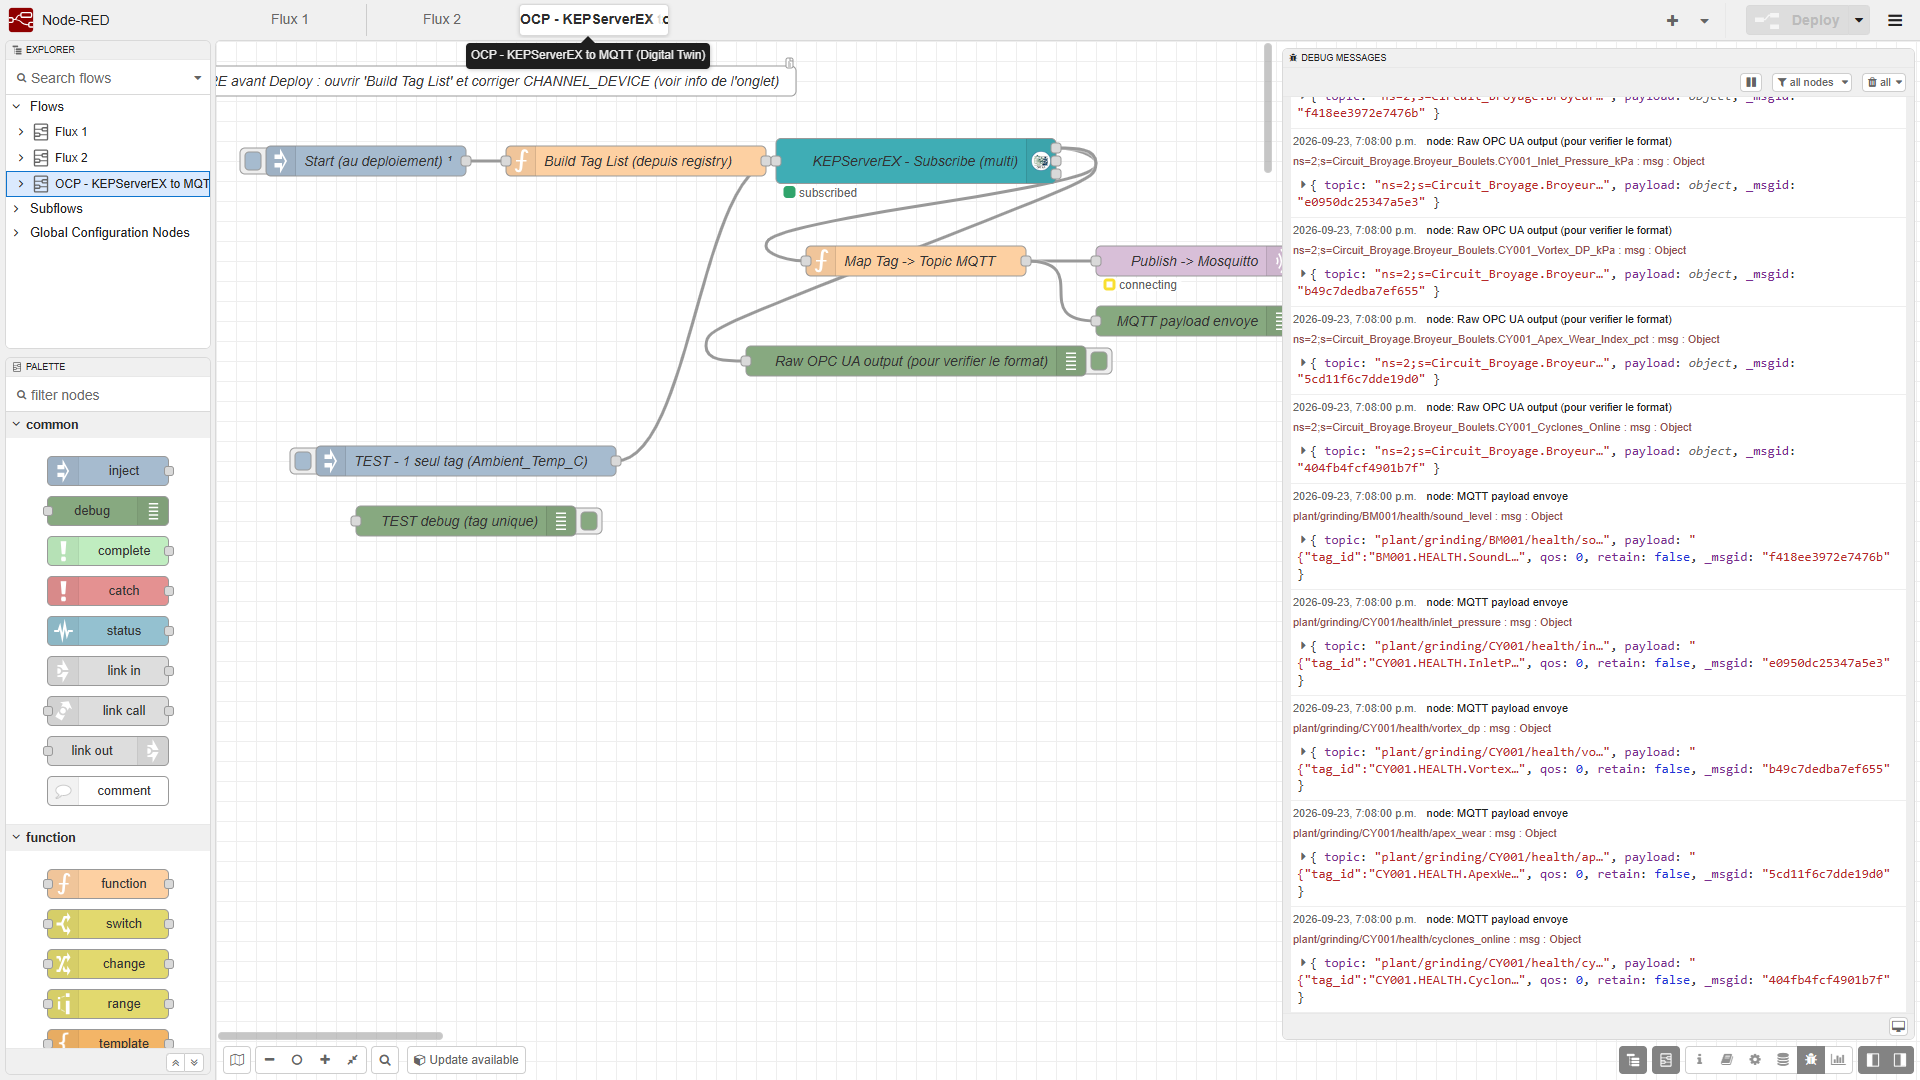
\includegraphics[width=\textwidth]{app_nodered}
\caption{Flux Node-RED «~OCP -- KEPServerEX to MQTT~» : abonnement OPC UA à KEPServerEX (état \textit{subscribed}), mise au format et publication MQTT ; à droite, les messages produits}
\label{fig:nodered}
\end{figure}

\subsection{Relecture des historiques}
La seconde source est un publieur Python, lancé dans son propre conteneur, qui rejoue les historiques du procédé :
\begin{itemize}
  \item 2\,880 mesures de procédé, une toutes les 15 minutes ;
  \item 43\,200 mesures de santé, une par minute.
\end{itemize}
Les deux fichiers couvrent le mois de juillet 2026. Le publieur s'appuie sur le registre des tags pour publier chaque colonne sur son topic. Il écoute aussi le topic de contrôle \texttt{plant/simulation/control}, ce qui permet de démarrer, suspendre ou accélérer la relecture depuis l'interface (jusqu'à 600 fois le temps réel).

\subsection*{Pourquoi OPC UA puis MQTT ?}
Les deux protocoles sont complémentaires plutôt que concurrents (tableau~\ref{tab:protocoles}). OPC UA~\cite{iec62541} est le standard d'accès aux automates : il décrit finement les données, mais repose sur un modèle client-serveur. MQTT~\cite{mqtt5} est un protocole de publication-abonnement très léger : un producteur publie une seule fois, et tous les services abonnés reçoivent le message. C'est le modèle idéal pour distribuer une même mesure à l'historien, aux calculs et à l'interface.

\begin{table}[H]
\centering
\caption{Comparaison des protocoles envisagés}
\label{tab:protocoles}
\begin{tabularx}{\textwidth}{lXXX}
\toprule
\textbf{Critère} & \textbf{OPC UA} & \textbf{MQTT} & \textbf{HTTP / REST} \\
\midrule
Modèle & Client-serveur (et pub/sub depuis la partie 14) & Publication-abonnement via broker & Requête-réponse \\
Surcoût réseau & Moyen & Très faible (en-tête fixe de 2 octets) & Élevé \\
Diffusion vers N services & N connexions & Une publication, N abonnés & N requêtes \\
Qualité de service & Session & 3 niveaux (QoS 0, 1, 2) & Aucune native \\
Usage dans le projet & KEPServerEX $\rightarrow$ Node-RED & Sources $\rightarrow$ backend & Interface $\rightarrow$ API \\
\bottomrule
\end{tabularx}
\end{table}

\section{Couche 2 : transport et traitement}
Le broker \textbf{Eclipse Mosquitto} reçoit les messages sur le port 1883. Sa persistance est activée et stockée dans un volume Docker.

Le \textbf{backend}, écrit en Python avec FastAPI~\cite{fastapi}, suit une architecture orientée domaines (\textit{Domain-Driven Design}). Chaque domaine regroupe sa logique métier, et les services sont injectés dans les routes de l'API :
\begin{itemize}
  \item \texttt{telemetry} : abonnement MQTT (\texttt{plant/grinding/\#}), état courant de chaque tag, trié par source, calcul des indicateurs dérivés et historien ;
  \item \texttt{simulation} : machine à états de la relecture (démarrage, pause, arrêt, vitesse) ;
  \item \texttt{assets} : fiches des équipements et historique des interventions ;
  \item \texttt{knowledge\_graph} : construction du graphe, accès à Neo4j et copilote Graph RAG ;
  \item \texttt{whatif} : simulateur What-If ;
  \item \texttt{auth} : authentification et rôles.
\end{itemize}

Pour chaque équipement, le domaine \texttt{telemetry} calcule des \textbf{indicateurs dérivés} à partir des mesures brutes : bilan de matière (débit entrant, débit sortant, écart), répartition sousverse/surverse des hydrocyclones, réduction de taille réalisée par le broyeur, et charge circulante.

\section{Couche 3 : stockage}
Aucune base ne répond seule à tous les besoins. Le projet associe donc plusieurs modes de stockage, chacun choisi pour un usage précis (tableau~\ref{tab:stockage}).

\begin{table}[H]
\centering
\caption{Stratégie de stockage et justification}
\label{tab:stockage}
\begin{tabularx}{\textwidth}{>{\raggedright\arraybackslash}p{2.6cm} >{\raggedright\arraybackslash}p{3.6cm} X}
\toprule
\textbf{Stockage} & \textbf{Contenu} & \textbf{Justification} \\
\midrule
Historien SQLite~\cite{sqlite} & Chaque message MQTT reçu & Base sans serveur, contenue dans un seul fichier : rien à installer, sauvegarde par simple copie. Le mode WAL autorise les lectures pendant l'écriture. \\
Neo4j~\cite{neo4j} & Équipements, lignes, capteurs, modes de défaillance, bons de travail & Les questions de topologie («~qu'y a-t-il en aval de ?~») sont des parcours de graphe, coûteux en jointures dans une base relationnelle. Un graphe en mémoire prend le relais si Neo4j est indisponible. \\
Fichiers CSV & Historiques du procédé et de la santé, fiches équipements, interventions, registre des tags & Source de vérité unique (dossier \texttt{data/}), partagée par le publieur, le backend et les modèles. \\
Fichiers joblib & Modèles entraînés & Évite de réentraîner à chaque démarrage ; le modèle est invalidé si les données ou sa version changent. \\
\bottomrule
\end{tabularx}
\end{table}

\subsection{L'historien de télémétrie}
\label{sec:historien}
Dans une première version, le backend ne gardait que les 100 dernières valeurs de chaque tag, en mémoire vive. Tout l'historique était donc perdu à chaque arrêt du poste. L'historien corrige ce défaut. Il enregistre chaque message dans la table \texttt{telemetry} d'un fichier SQLite, avec les champs suivants :
\begin{itemize}
  \item l'horodatage de mesure et l'horodatage de réception ;
  \item le topic, le tag, la valeur, l'unité et la qualité ;
  \item la source et le domaine ;
  \item le message JSON complet.
\end{itemize}
Deux index accélèrent les recherches par tag et par période. Pour ne jamais ralentir la réception MQTT, le rappel de réception se contente de placer le message dans une file d'attente, et un fil d'exécution dédié l'écrit ensuite sur le disque par lots. À l'arrêt, la file est vidée avant la fermeture. Au démarrage, les 100 derniers messages de chaque tag sont rechargés en mémoire, si bien que les courbes reprennent là où elles s'étaient arrêtées. Trois routes de l'API exposent l'historique : \texttt{/historian/stats}, \texttt{/historian/query} et \texttt{/historian/export.csv}.

\section{Couche 4 : intelligence artificielle}

\begin{figure}[H]
\centering
\begin{tikzpicture}[
  e/.style={boite,text width=3.5cm,font=\scriptsize},
  m/.style={boite,draw=rouge,fill=rougeclair,text width=3cm,font=\scriptsize},
  s/.style={boite,draw=vert,fill=vertclair,text width=3.5cm,font=\scriptsize}]
  \node[e] (e1) at (0,0) {\textbf{8 entrées réglables}\\alimentation, eau, vitesses, consigne de niveau};
  \node[m] (m1) at (4.8,0) {\textbf{Forêt aléatoire}\\multi-sorties};
  \node[s] (s1) at (9.6,0) {\textbf{23 grandeurs aval}\\prédites + $R^2$ par sortie};
  \node[e] (e2) at (0,-2) {\textbf{Question en langage naturel}\\+ graphe, télémétrie, interventions};
  \node[m] (m2) at (4.8,-2) {\textbf{Graph RAG}\\LLM Gemini ou moteur local};
  \node[s] (s2) at (9.6,-2) {\textbf{Réponse argumentée}\\diagnostic, recommandation};
  \node[e] (e3) at (0,-4) {\textbf{Mesures en ligne}\\débits, densités, santé};
  \node[m] (m3) at (4.8,-4) {\textbf{XGBoost}\\régression};
  \node[s] (s3) at (9.6,-4) {\textbf{P80 estimé}\\en continu};
  \foreach \i in {1,2,3} {\draw[fleche] (e\i)--(m\i); \draw[fleche] (m\i)--(s\i);}
\end{tikzpicture}
\caption{Entrées, modèles et sorties de la couche d'intelligence artificielle}
\label{fig:ia}
\end{figure}

\paragraph{Simulateur What-If.} Une forêt aléatoire multi-sorties~\cite{breiman2001} (scikit-learn~\cite{sklearn} ; 100 arbres, profondeur maximale 22) prédit 23 grandeurs aval du circuit à partir de 8 entrées qu'un opérateur peut réellement régler en amont :
\begin{itemize}
  \item débit, teneur BPL, P80 et fraction solide de l'alimentation ;
  \item débit d'eau d'appoint ;
  \item vitesse de la pompe et vitesse du broyeur ;
  \item consigne de niveau du bac.
\end{itemize}
Ces 23 grandeurs couvrent les cyclones, le broyage, la qualité, la santé du broyeur et celle de la pompe. Le modèle est entraîné sur l'historique fusionné, puis mis en cache sur disque. Pour chaque sortie, l'interface affiche la valeur actuelle, la valeur prédite, l'écart entre les deux et le $R^2$ du modèle, afin que l'utilisateur sache quelle confiance accorder à chaque prédiction.

\paragraph{Copilote Graph RAG.} Le copilote suit le principe du Graph RAG~\cite{edge2024,lewis2020} en quatre étapes :
\begin{enumerate}
  \item il repère dans la question les équipements concernés ;
  \item il extrait le sous-graphe correspondant ;
  \item il récupère la télémétrie courante et les interventions de maintenance de ces équipements ;
  \item il assemble ce contexte dans une requête à l'API Google Gemini.
\end{enumerate}
Si l'API ne répond pas, un \textbf{moteur local déterministe} rédige la réponse à partir du même contexte. Le copilote reste ainsi utilisable sans connexion.

\paragraph{Capteur virtuel XGBoost.} Un modèle XGBoost~\cite{chen2016} estime le P80 de la surverse à partir des seules mesures disponibles en ligne. Il a été développé et évalué hors ligne ; son protocole et ses résultats font l'objet de la section~\ref{sec:xgboost}.

\section{Couche 5 : interface utilisateur}
L'interface est une \gls{spa} développée avec React 19~\cite{react} et Vite. Le graphe de connaissances est rendu avec vis-network, la vue 3D avec React Three Fiber~\cite{r3f} (Three.js), et les graphiques avec Recharts. La charte graphique applique les principes de la norme ISA-101~\cite{isa101} : un fond sombre et neutre, et des couleurs vives réservées aux situations anormales, afin que l'attention de l'opérateur se porte sur l'essentiel.

\section{Modèle de données}

\subsection{Registre des signaux}
Le fichier \texttt{tag\_mapping\_registry.csv} décrit les 45 signaux du circuit. Pour chacun, il donne la colonne source, l'identifiant du tag, le topic MQTT, l'équipement, la ligne, l'unité, le type et la période d'échantillonnage. Ces signaux se répartissent en deux domaines (tableau~\ref{tab:tags}) :
\begin{itemize}
  \item la \textbf{santé} des équipements, acquise chaque minute ;
  \item le \textbf{procédé} (bilans de matière et qualité), acquis toutes les 15 minutes.
\end{itemize}

{\footnotesize
\begin{longtable}{l >{\raggedright\arraybackslash}p{6.3cm} >{\raggedright\arraybackslash}p{4.1cm} >{\centering\arraybackslash}p{2.1cm}}
\caption{Registre des signaux de télémétrie}\label{tab:tags}\\
\toprule
\textbf{Équip.} & \textbf{Tag} & \textbf{Grandeur} & \textbf{Unité} \\
\midrule
\endfirsthead
\toprule
\textbf{Équip.} & \textbf{Tag} & \textbf{Grandeur} & \textbf{Unité} \\
\midrule
\endhead
\bottomrule
\endfoot
\rowcolor{grisclair}\multicolumn{4}{c}{\textbf{Domaine santé -- période 1 min (21 tags)}} \\
Circuit & \texttt{CIRCUIT.ENV.AmbientTemp} & Température ambiante & °C \\
PB\_001 & \texttt{PB001.HEALTH.\{Level, LevelSetpoint, SumpTemp\}} & Niveau, consigne, température du bac & \%, \%, °C \\
SP\_001 & \texttt{SP001.HEALTH.\{MotorCurrent, MotorPower, DischargePressure, Speed, BearingTemp, Vibration\}} & Courant, puissance, pression de refoulement, vitesse, température palier, vibration & A, kW, kPa, tr/min, °C, mm/s \\
BM\_001 & \texttt{BM001.HEALTH.\{PowerDraw, MotorCurrent, SpeedPctCritical, BearingDETemp, BearingNDETemp, Vibration, SoundLevel\}} & Puissance, courant, vitesse, températures paliers, vibration, niveau sonore & kW, A, \% crit., °C, mm/s, dB \\
CY\_001 & \texttt{CY001.HEALTH.\{InletPressure, VortexDP, ApexWear, CyclonesOnline\}} & Pression d'entrée, pression différentielle, usure de l'apex, cyclones en service & kPa, kPa, \%, nombre \\
\rowcolor{grisclair}\multicolumn{4}{c}{\textbf{Domaine procédé -- période 15 min (24 tags)}} \\
PB\_001 & \texttt{PB001.IN.\{SolidFlow, BPL, P80, SolidFraction\}} & Alimentation fraîche & t/h, \%, µm, \% \\
 & \texttt{PB001.WATER.\{SolidFlow, SolidFraction\}} & Eau d'appoint & t/h, \% \\
CY\_001 & \texttt{CY001.FEED.\{SolidFlow, BPL, P80, SolidFraction\}} & Alimentation cyclones & t/h, \%, µm, \% \\
 & \texttt{CY001.OF.\{\ldots\}} et \texttt{CY001.UF.\{\ldots\}} & Surverse et sousverse & idem \\
BM\_001 & \texttt{BM001.DISCH.\{SolidFlow, BPL, P80, SolidFraction\}} & Décharge broyeur & t/h, \%, µm, \% \\
Circuit & \texttt{CIRCUIT.KPI.\{CirculatingLoad, ReductionRatio\}} & Charge circulante, rapport de réduction & \%, -- \\
\end{longtable}
}

\subsection{Asymétrie temporelle des flux}
\label{sec:asymetrie}
Les deux domaines n'arrivent pas au même rythme : il y a une mesure de procédé pour quinze mesures de santé. Or le calcul d'un bilan de matière, comme l'apprentissage d'un modèle, exige des valeurs cohérentes dans le temps. Le fournisseur de données du backend fusionne donc les deux flux par une \textbf{jointure temporelle} (\textit{as-of join}) : chaque mesure de santé est associée à la dernière mesure de procédé connue à cet instant (figure~\ref{fig:asym}).

\begin{figure}[H]
\centering
\begin{tikzpicture}[x=0.36cm]
  \node[font=\scriptsize\bfseries,anchor=east,rouge] at (-0.3,1) {Santé (1 min)};
  \node[font=\scriptsize\bfseries,anchor=east,bleu] at (-0.3,0) {Procédé (15 min)};
  \draw[gris] (0,1) -- (30.5,1); \draw[gris] (0,0) -- (30.5,0);
  \foreach \t in {0,...,30} \fill[rouge] (\t,1) circle (2pt);
  \foreach \t in {0,15,30} {\fill[bleu] (\t,0) circle (3.5pt);}
  \foreach \t in {1,4,...,13} \draw[-{Stealth[length=1.2mm]},vert] (0,0.12) to[bend left=10] (\t,0.88);
  \foreach \t in {16,19,...,28} \draw[-{Stealth[length=1.2mm]},vert] (15,0.12) to[bend left=10] (\t,0.88);
  \draw[-{Stealth},gris] (0,-0.8) -- (31,-0.8) node[right,font=\scriptsize]{temps (min)};
  \foreach \t in {0,15,30} \node[below,font=\scriptsize] at (\t,-0.8) {\t};
  \node[font=\scriptsize,vert,align=center] at (15,-1.8) {chaque mesure de santé reçoit la dernière mesure de procédé connue};
\end{tikzpicture}
\caption{Fusion de flux échantillonnés à des fréquences différentes (jointure temporelle)}
\label{fig:asym}
\end{figure}

\subsection{Structure des topics MQTT}
Les topics suivent une hiérarchie stricte :
\begin{center}\texttt{plant/grinding/<équipement>/<domaine>/<point>/<grandeur>}\end{center}
Par exemple, \nolinkurl{plant/grinding/PB001/process/in/solid_flow} transporte le débit solide de l'alimentation fraîche. Cette hiérarchie permet aux services de s'abonner par famille grâce aux jokers MQTT (\texttt{+} et \texttt{\#})~\cite{mqtt5}. Par exemple, \nolinkurl{plant/grinding/BM001/health/#} donne accès à toute la santé du broyeur.

\subsection{Format des messages}
Chaque message est un objet JSON autodescriptif (code~\ref{lst:payload}). Il contient la valeur, l'identifiant du tag, l'unité, l'horodatage, la qualité, le domaine et la \textbf{source}. Ce dernier champ permet au backend et à l'interface de distinguer les données rejouées (\texttt{csv\_replay\_mqtt}) de celles venant de la chaîne OPC UA (\texttt{nodered\_opcua}).

\begin{lstlisting}[caption={Exemple de message publié par la relecture},label={lst:payload}]
{
  "tag_id": "PB001.IN.SolidFlow",
  "value": 463.439,
  "unit": "t/h",
  "timestamp": "2026-07-01 00:00:00",
  "quality": "SIM",
  "domain": "process",
  "source": "csv_replay_mqtt"
}
\end{lstlisting}

\section{Cycle de vie d'une donnée}

\begin{figure}[H]
\centering
\begin{tikzpicture}[et/.style={boite,text width=3cm,font=\scriptsize,minimum height=1.3cm}]
  \node[et] (a) at (0,2.4) {\textbf{1. Mesure}\\tag KEPServerEX ou ligne d'historique};
  \node[et] (b) at (4.8,2.4) {\textbf{2. Publication}\\Node-RED ou publieur $\rightarrow$ MQTT};
  \node[et] (c) at (9.6,2.4) {\textbf{3. Réception}\\état en mémoire + historien};
  \node[et,draw=rouge,fill=rougeclair] (d) at (9.6,0) {\textbf{4. Calcul}\\bilans, indicateurs, modèles};
  \node[et,draw=violet,fill=violet!8] (e) at (4.8,0) {\textbf{5. Affichage}\\synoptique, fiches, 3D};
  \node[et,draw=vert,fill=vertclair] (f) at (0,0) {\textbf{6. Décision}\\opérateur, ingénieur, copilote};
  \draw[fleche] (a)--(b); \draw[fleche] (b)--(c); \draw[fleche] (c)--(d);
  \draw[fleche] (d)--(e); \draw[fleche] (e)--(f);
  \draw[fleche,dashed] (f)--node[left,font=\tiny,align=right]{action sur\\le procédé}(a);
\end{tikzpicture}
\caption{Cycle de vie d'une donnée dans le jumeau numérique}
\label{fig:cycle}
\end{figure}

La dernière étape reste humaine : le système informe et recommande, mais n'agit pas directement sur le procédé. C'est un choix délibéré pour une preuve de concept, qui correspond à la notion d'ombre numérique présentée au chapitre~\ref{chap:etatart}.

\section{Conclusion}
L'architecture sépare nettement l'acquisition, le traitement, le stockage, l'IA et la restitution, et chaque brique a été choisie pour un usage précis. Le découplage par MQTT permet de brancher indifféremment la relecture, la chaîne OPC UA ou, à terme, une installation réelle. Le chapitre suivant présente la mise en œuvre et les résultats obtenus.

\chapter{Réalisation et résultats}
\label{chap:realisation}

\section{Introduction}
Ce chapitre présente l'environnement de développement et les interfaces réalisées, puis l'évaluation chiffrée du prototype. Il se termine par une analyse honnête de ses limites. Toutes les captures d'écran ont été prises sur l'application en fonctionnement.

\section{Environnement technique}

\begin{table}[H]
\centering
\caption{Technologies utilisées}
\label{tab:techno}
\begin{tabularx}{\textwidth}{l X}
\toprule
\textbf{Domaine} & \textbf{Outils} \\
\midrule
Acquisition & KEPServerEX V6 (OPC UA)~\cite{kepware}, Node-RED et \texttt{node-red-contrib-opcua}~\cite{nodered} \\
Transport & Eclipse Mosquitto 2.0 (MQTT)~\cite{mqtt5}, paho-mqtt \\
Back-end & Python, FastAPI~\cite{fastapi}, pandas, PyJWT, bcrypt \\
Stockage & SQLite~\cite{sqlite}, Neo4j 5~\cite{neo4j}, fichiers CSV \\
Apprentissage & scikit-learn~\cite{sklearn}, XGBoost~\cite{chen2016}, joblib \\
IA générative & API Google Gemini, Graph RAG~\cite{edge2024} \\
Front-end & React 19~\cite{react}, Vite, React Three Fiber~\cite{r3f}, vis-network, Recharts \\
Déploiement & Docker Compose~\cite{merkel2014} : 5 services (broker, Neo4j, backend, publieur, frontend) \\
\bottomrule
\end{tabularx}
\end{table}

\section{Interfaces réalisées}

\subsection{Authentification}
L'accès passe par une page de connexion (figure~\ref{fig:login}). Le backend vérifie le mot de passe haché avec bcrypt, puis délivre un jeton \gls{jwt} valable 8 heures. Chaque page de l'application est protégée : sans jeton valide, l'utilisateur est renvoyé vers la connexion.

\begin{figure}[H]
\centering
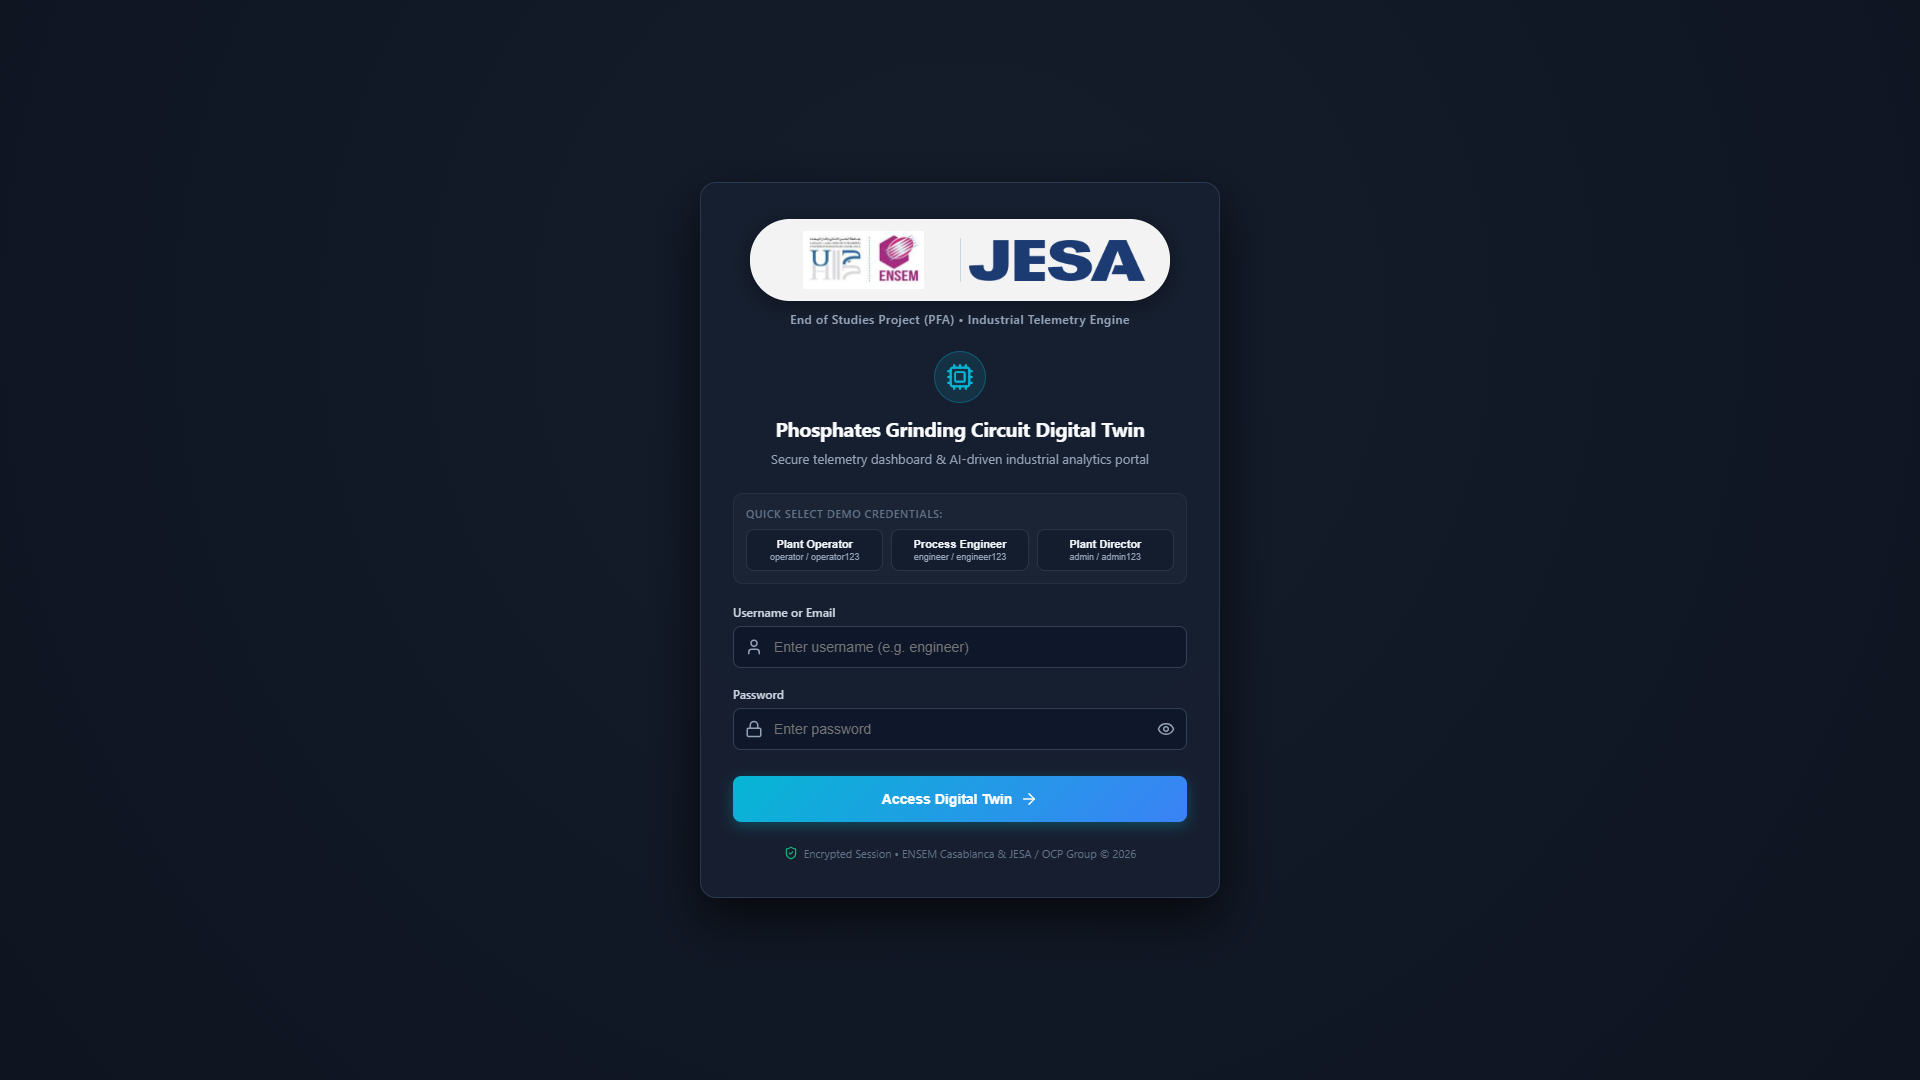
\includegraphics[width=0.8\textwidth]{app_login}
\caption{Page de connexion, avec les trois profils de démonstration}
\label{fig:login}
\end{figure}

\subsection{Synoptique et graphe de connaissances}
La vue principale juxtapose le schéma du circuit et le graphe de connaissances (figure~\ref{fig:home}). Une barre de pilotage permet de lancer la relecture et de choisir sa vitesse. Elle donne aussi accès aux panneaux de chaque source de données et au simulateur What-If.

\begin{figure}[H]
\centering
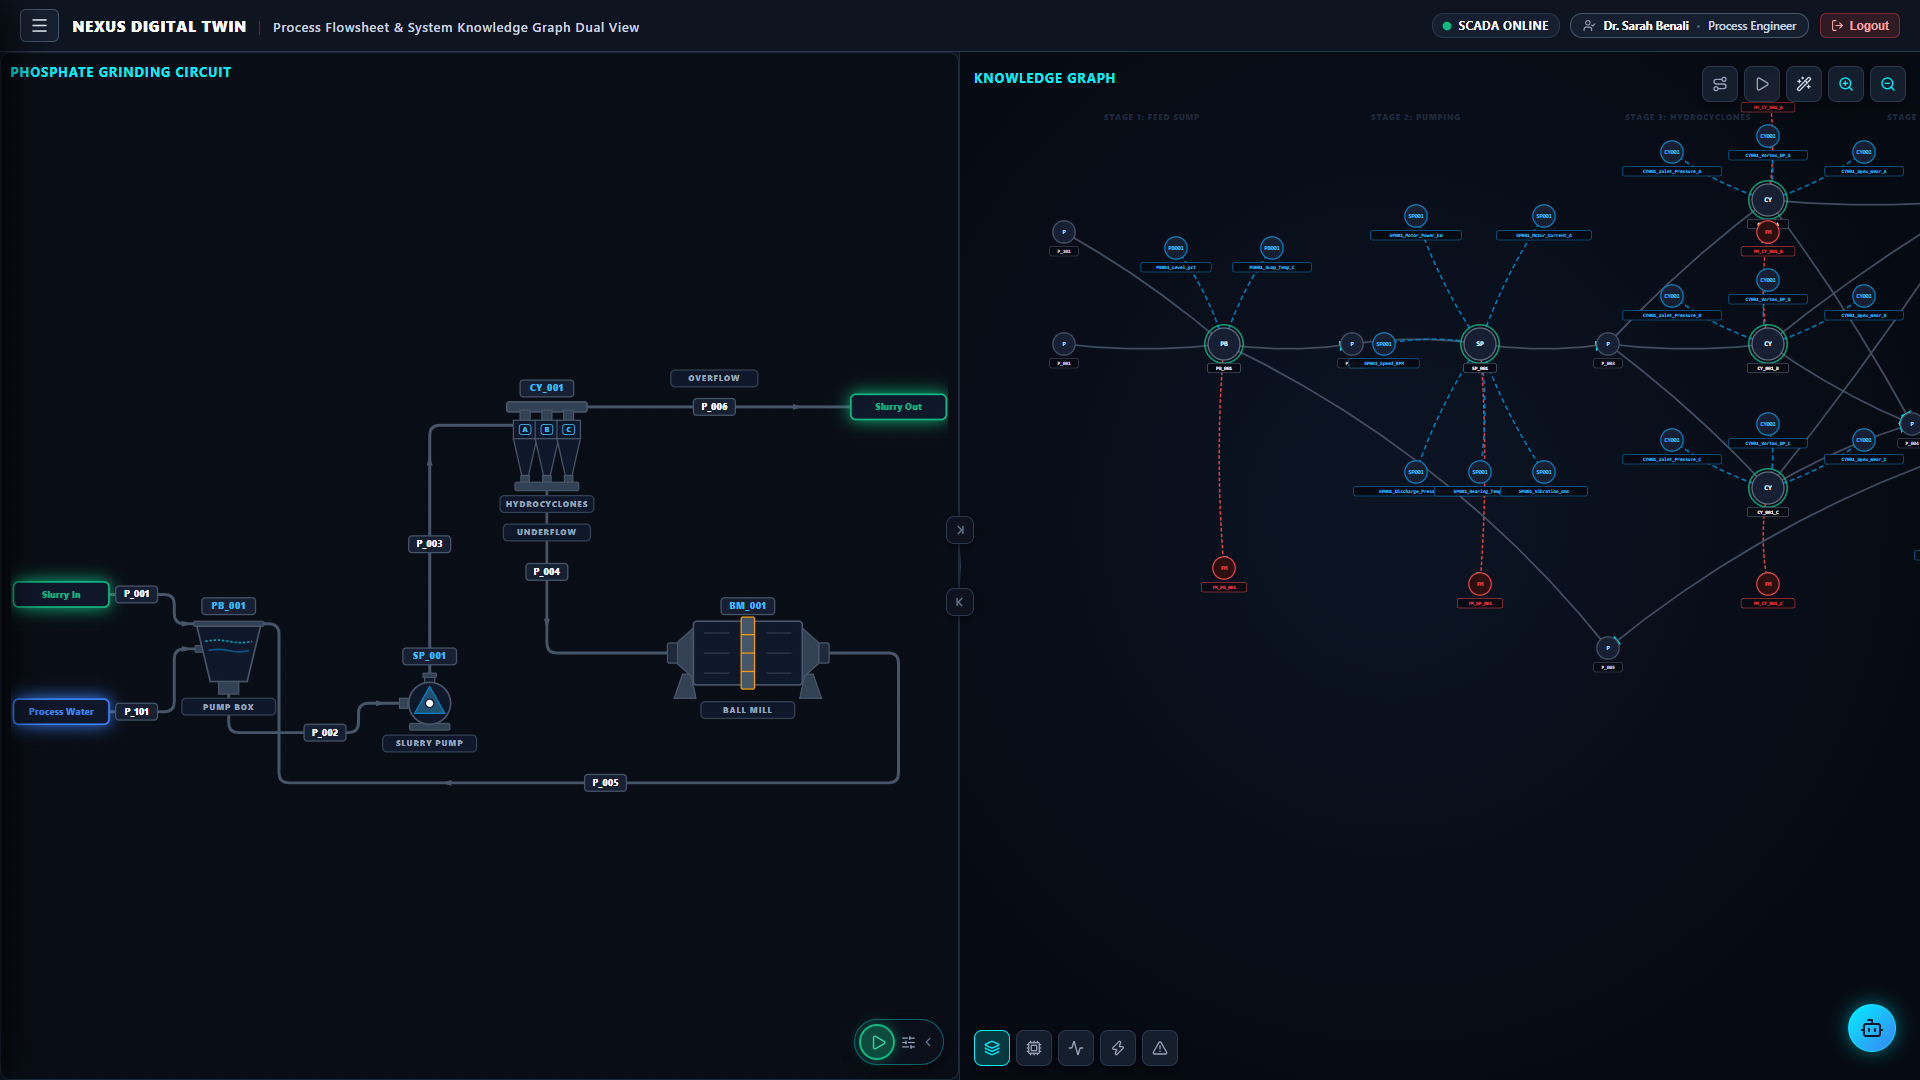
\includegraphics[width=\textwidth]{app_home}
\caption{Vue double : synoptique du circuit (à gauche) et graphe de connaissances (à droite)}
\label{fig:home}
\end{figure}

Pendant la relecture, les lignes s'animent selon les débits reçus, et chaque équipement s'illumine selon son état (figure~\ref{fig:flowsheet}).

\begin{figure}[H]
\centering
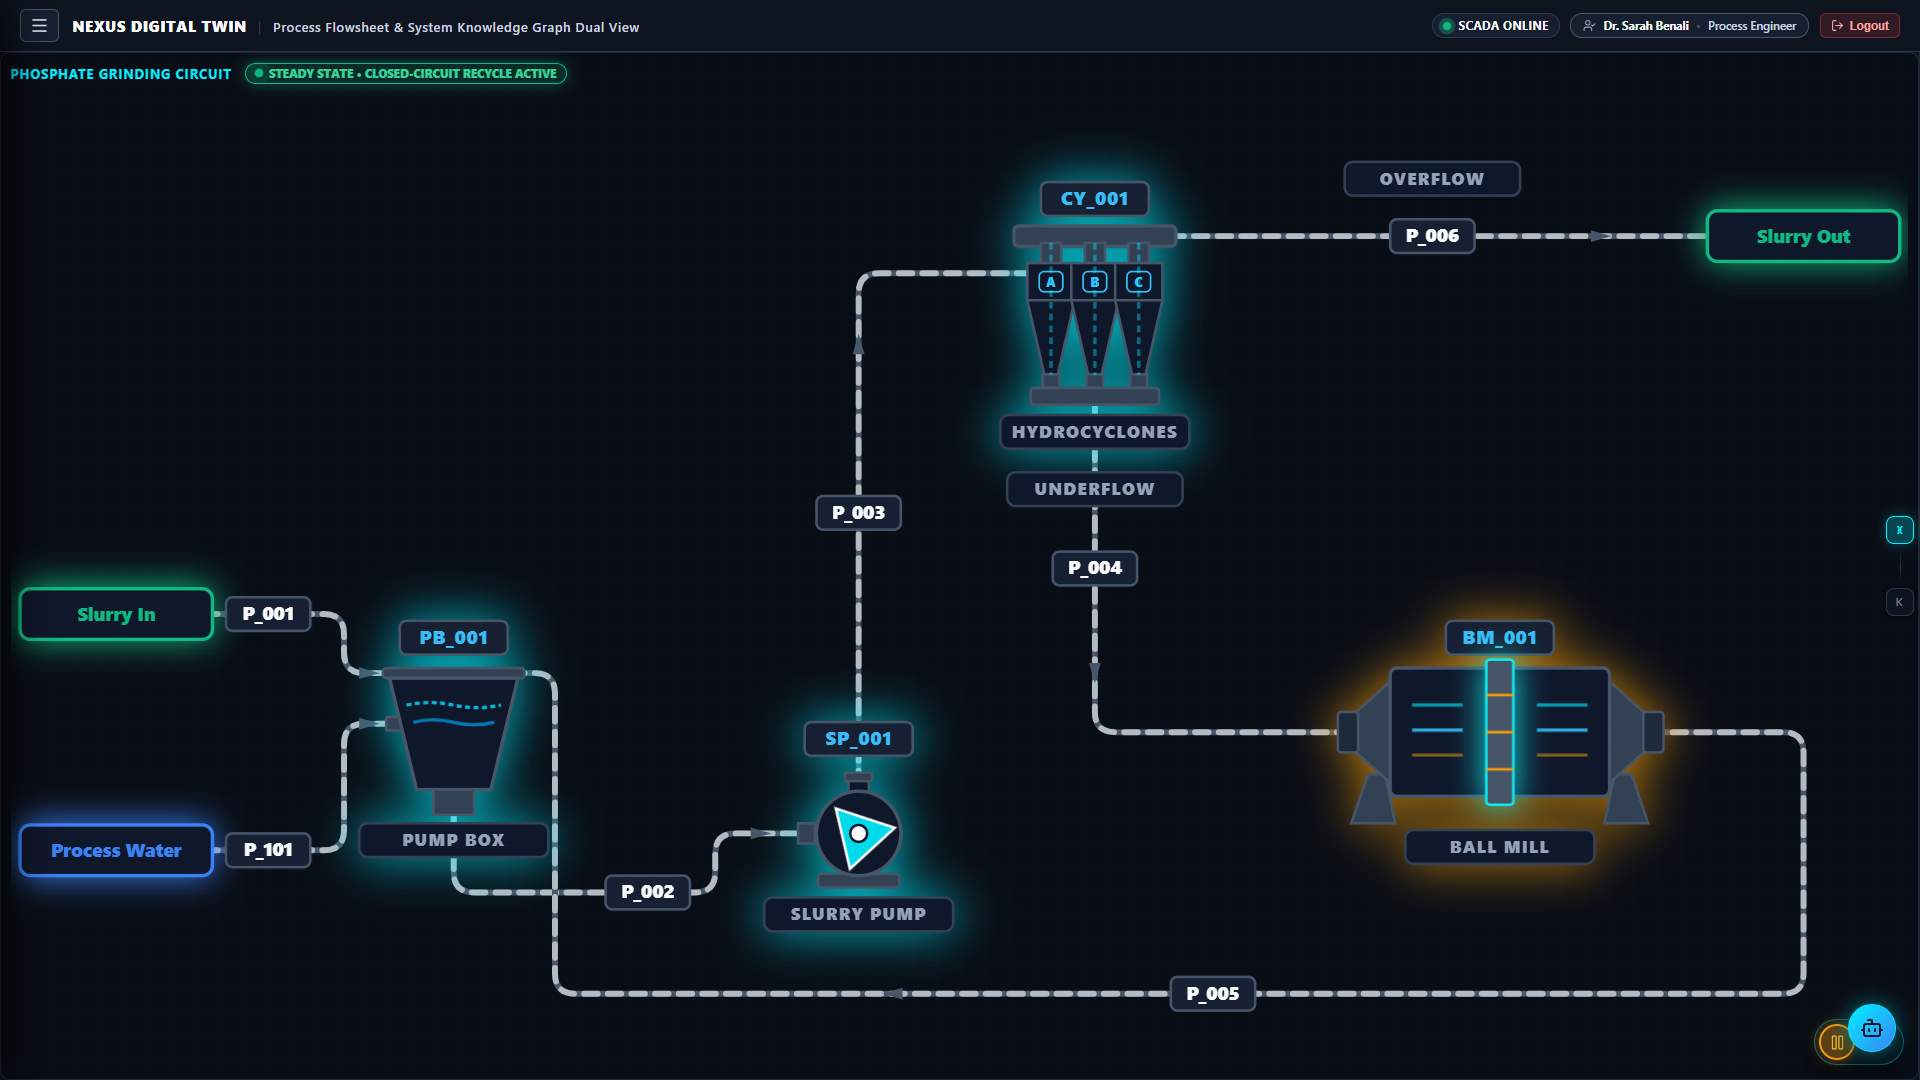
\includegraphics[width=\textwidth]{app_flowsheet_full}
\caption{Synoptique en plein écran pendant la relecture}
\label{fig:flowsheet}
\end{figure}

\subsection{Fiche d'un équipement}
Un clic sur un équipement ouvre sa fiche (figure~\ref{fig:drawer}). Pour le broyeur BM\_001, elle affiche :
\begin{itemize}
  \item la télémétrie en direct : puissance, courant, vitesse, températures des paliers, vibration, niveau sonore ;
  \item les indicateurs dérivés calculés par le backend : réduction de taille, débits entrant et sortant, écart de débit.
\end{itemize}
Le graphe se centre alors automatiquement sur cet équipement et met en évidence ses liens : capteurs (\texttt{MONITORS}), lignes (\texttt{FEEDS\_INTO}, \texttt{DISCHARGES\_TO}) et risques (\texttt{RISKS}).

\begin{figure}[H]
\centering
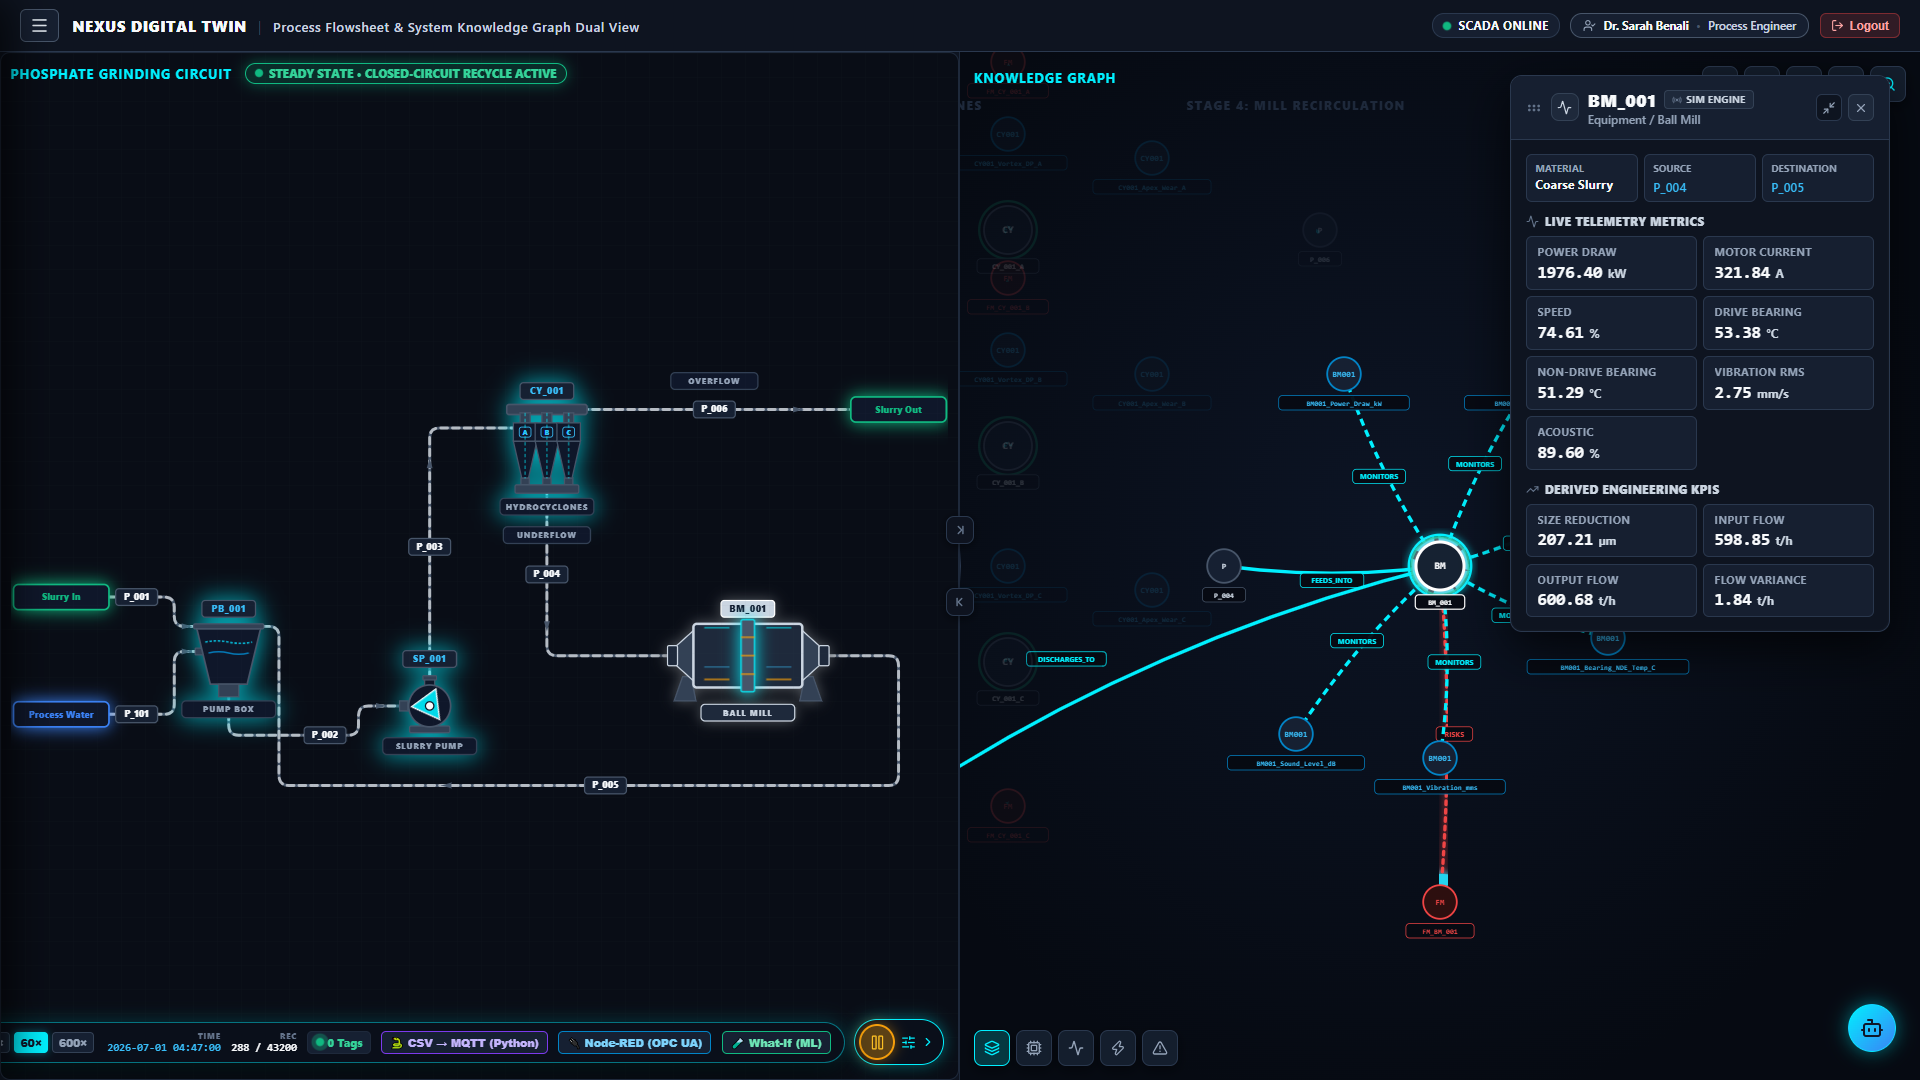
\includegraphics[width=\textwidth]{app_drawer_bm}
\caption{Fiche du broyeur BM\_001 : télémétrie en direct, indicateurs dérivés et voisinage dans le graphe}
\label{fig:drawer}
\end{figure}

Le graphe de connaissances compte \textbf{69 nœuds et 129 relations}, répartis ainsi :
\begin{itemize}
  \item 6 équipements, 7 lignes et 15 capteurs ;
  \item 6 modes de défaillance ;
  \item 29 bons de travail et 6 techniciens.
\end{itemize}
Des filtres isolent chaque famille de nœuds, et un mode de parcours trace le chemin d'une cause à ses effets.

\subsection{Simulateur What-If}
Le panneau What-If (figure~\ref{fig:whatif}) propose un curseur pour chacune des 8 entrées réglables. À chaque modification, il affiche pour chaque grandeur aval :
\begin{itemize}
  \item la valeur actuelle et la valeur prédite ;
  \item l'écart entre les deux ;
  \item le $R^2$ du modèle sur cette grandeur. Un badge orange signale une prédiction moins fiable, par exemple sur les pressions des cyclones.
\end{itemize}

\begin{figure}[H]
\centering
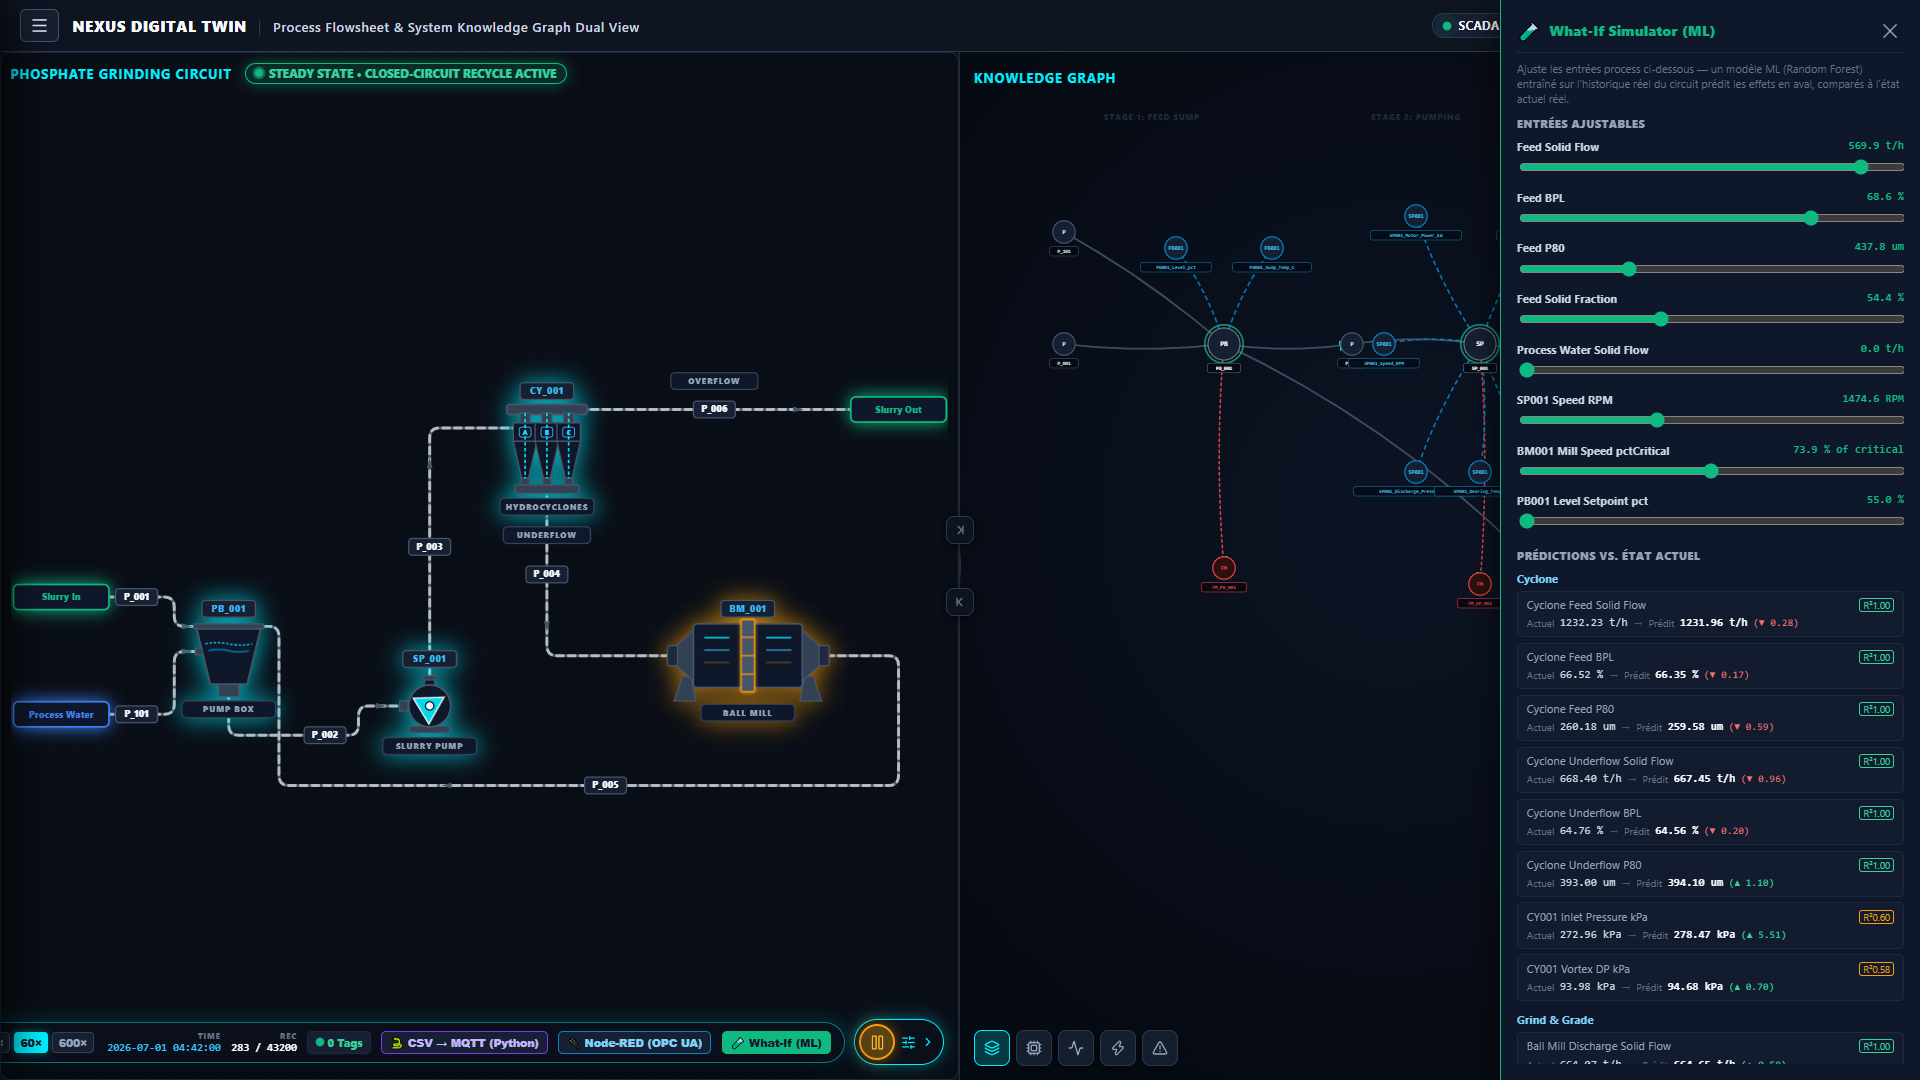
\includegraphics[width=\textwidth]{app_whatif}
\caption{Simulateur What-If : entrées réglables et prédictions comparées à l'état actuel}
\label{fig:whatif}
\end{figure}

\subsection{Vue 3D}
La vue 3D (figure~\ref{fig:3d}) reproduit l'implantation du circuit : bac, pompe, batterie de trois hydrocyclones, broyeur et tuyauteries. Au-dessus de chaque équipement, une étiquette affiche sa grandeur clé en direct : niveau du bac, pression de refoulement de la pompe, débit d'alimentation des cyclones, puissance du broyeur.

\begin{figure}[H]
\centering
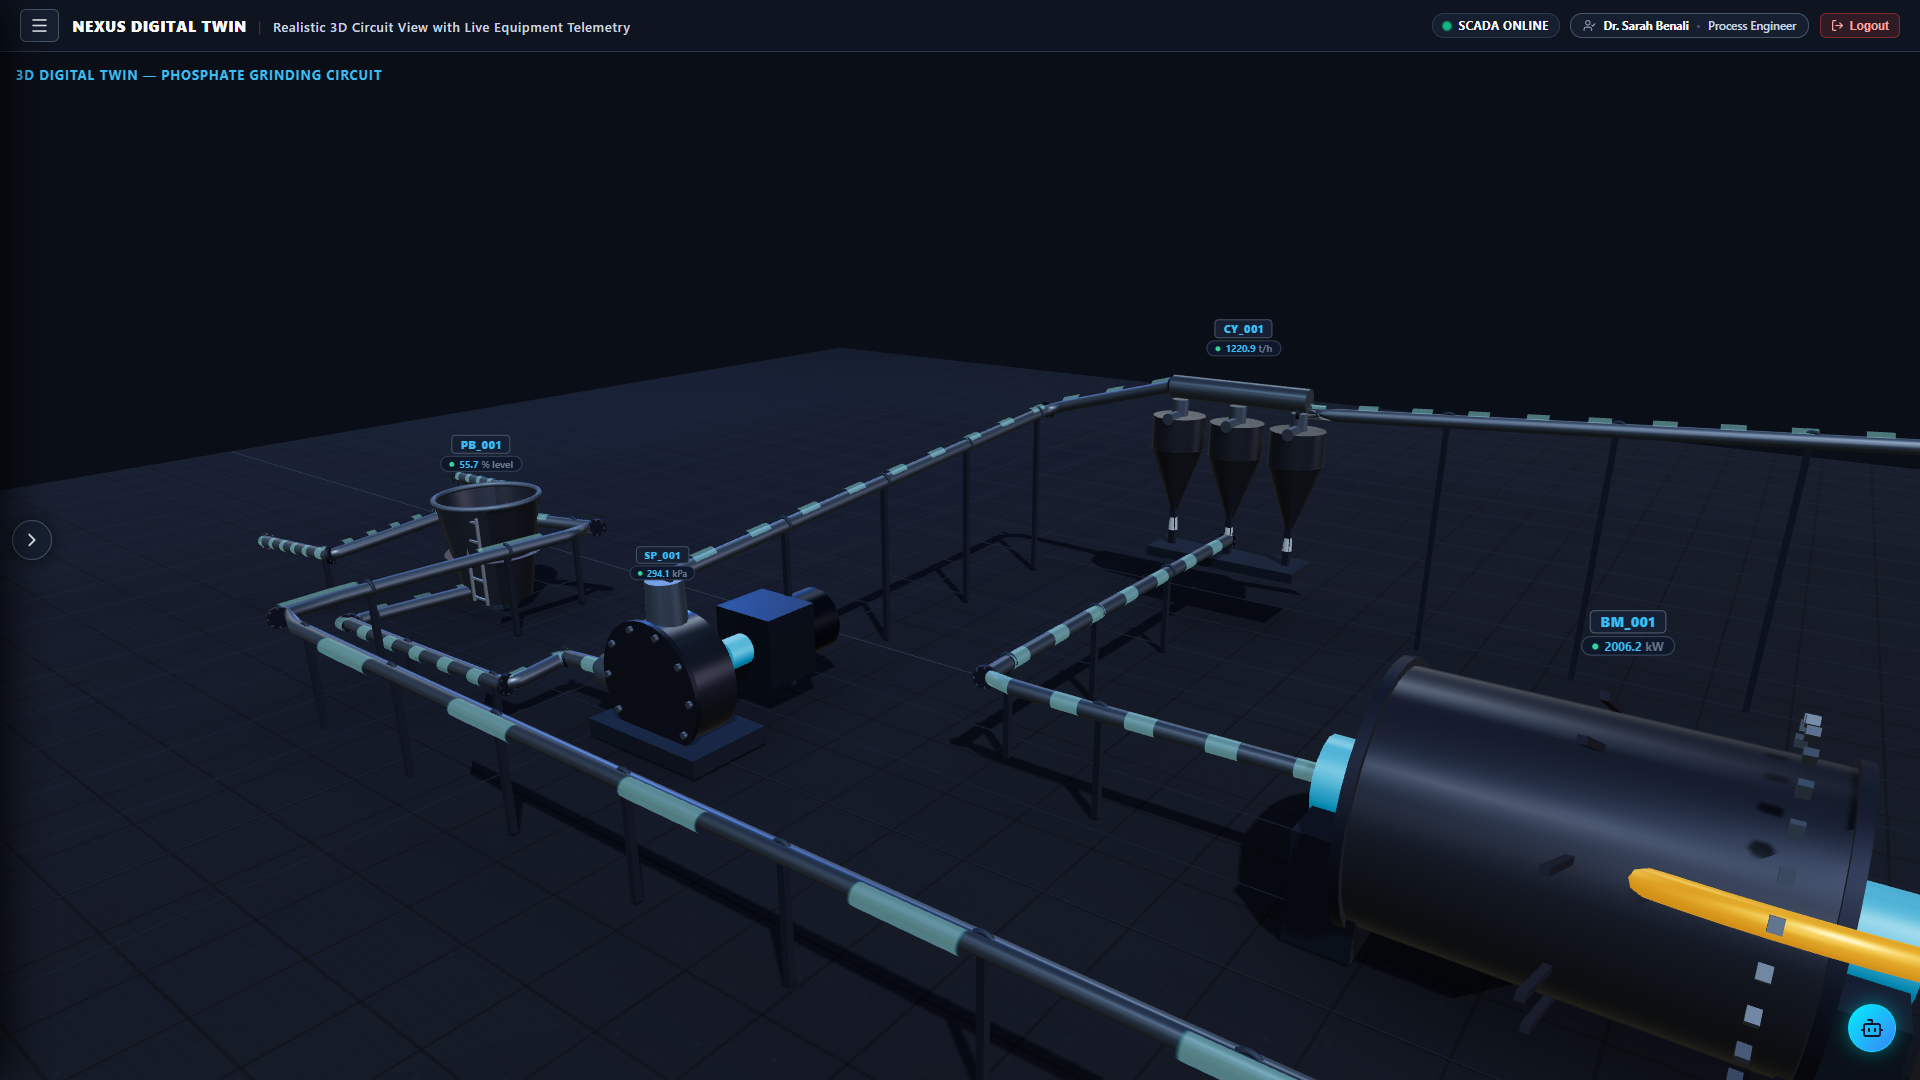
\includegraphics[width=\textwidth]{app_view3d}
\caption{Vue 3D du circuit réalisée avec React Three Fiber}
\label{fig:3d}
\end{figure}

\subsection{Maintenance et fiabilité}
La page de maintenance (figure~\ref{fig:maint}) résume l'état du parc : nombre d'équipements, interventions en retard, équipements critiques et MTBF moyen. Elle donne aussi accès à chaque équipement, avec le nombre de jours restant avant sa prochaine intervention. La fiche détaillée (figure~\ref{fig:maintpump}) présente :
\begin{itemize}
  \item les données constructeur de l'équipement ;
  \item la dernière intervention et la prochaine échéance ;
  \item l'état de l'équipement, avec son MTBF et son MTTR ;
  \item l'état de ses composants critiques.
\end{itemize}
Un lien ouvre l'historique complet des interventions (31 bons de travail au total).

\begin{figure}[H]
\centering
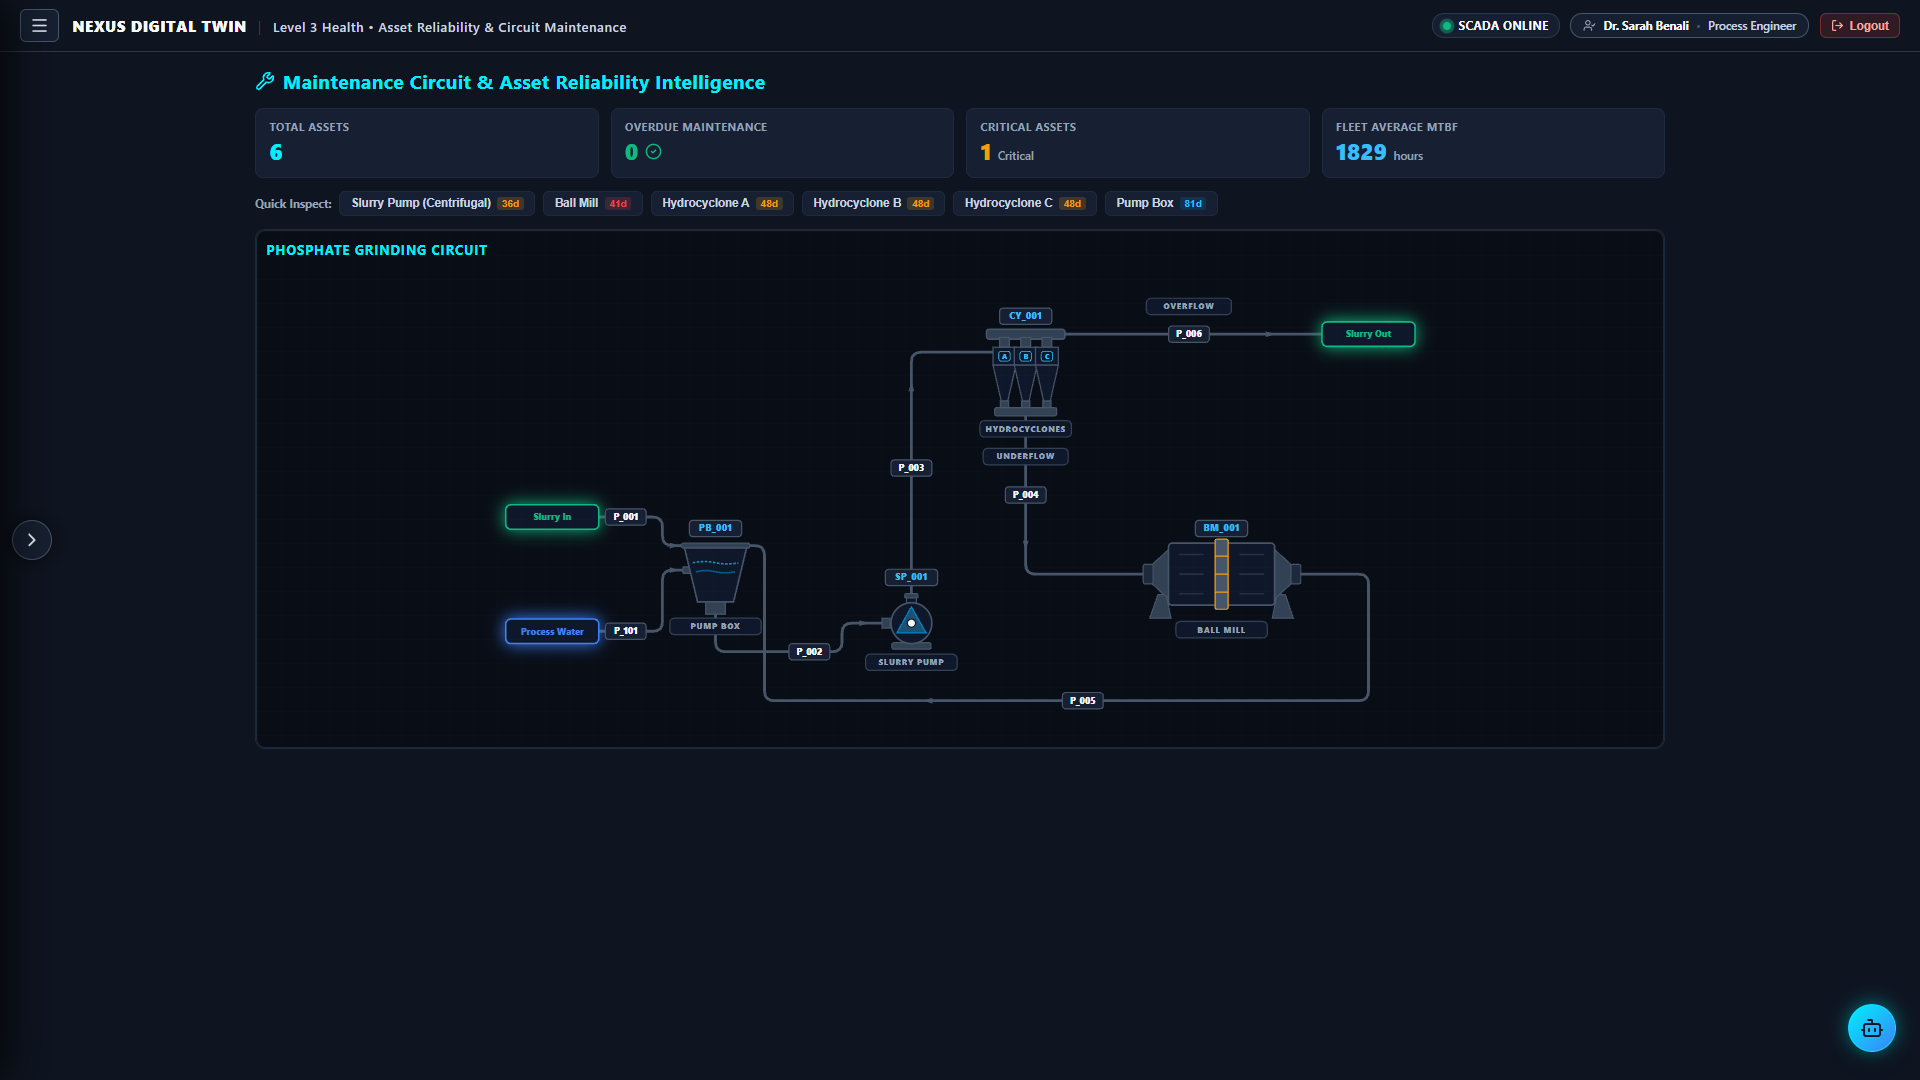
\includegraphics[width=\textwidth]{app_maintenance}
\caption{Tableau de bord de maintenance et de fiabilité}
\label{fig:maint}
\end{figure}

\begin{figure}[H]
\centering
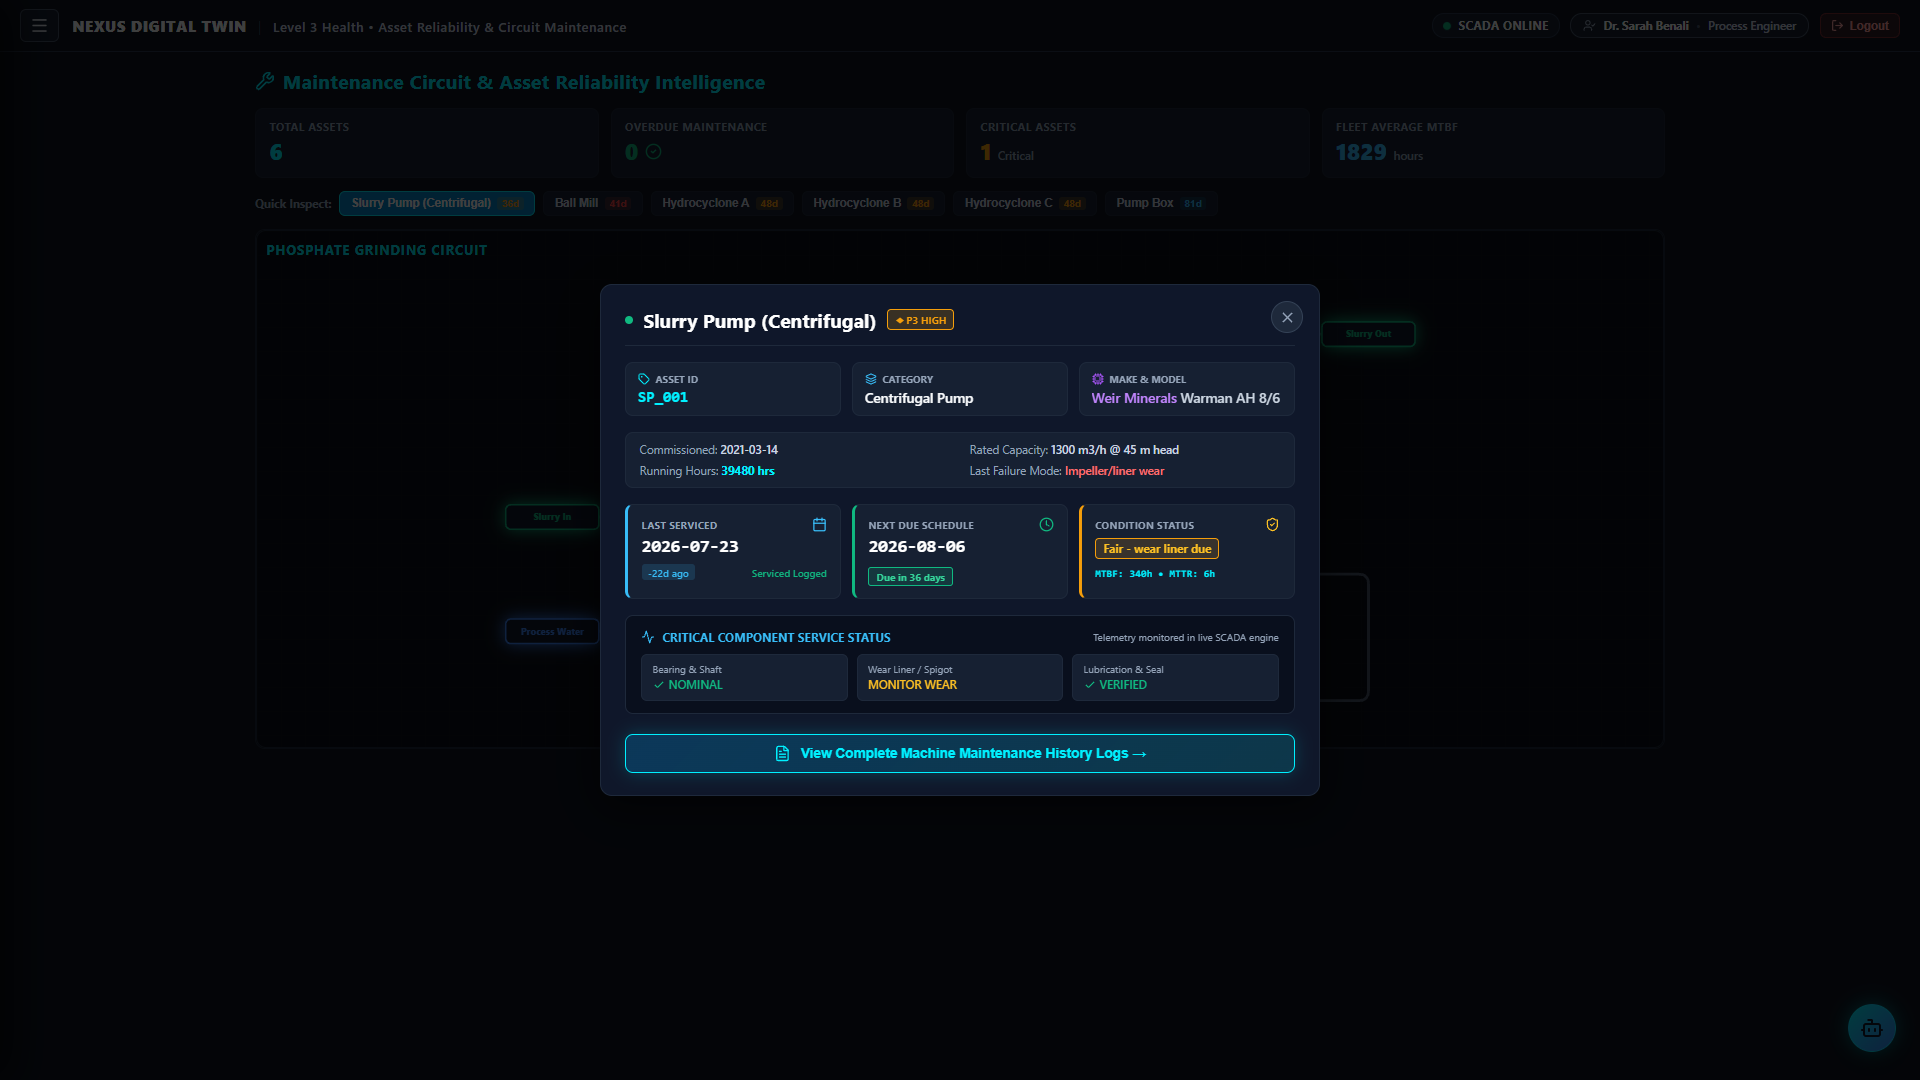
\includegraphics[width=\textwidth]{app_maintenance_pump}
\caption{Fiche de maintenance de la pompe SP\_001 (criticité haute, revêtement d'usure à remplacer)}
\label{fig:maintpump}
\end{figure}

\subsection{Copilote IA}
Le copilote (figure~\ref{fig:copilot}) est une fenêtre flottante disponible sur toutes les pages. Il propose des questions types, et chaque réponse indique le moteur utilisé et le nombre d'entités du graphe mobilisées. Dans l'exemple ci-dessous, pris hors connexion à l'API Gemini, le moteur local a construit sa réponse à partir de 15 entités. On y retrouve la vitesse du broyeur (74,05\,\% de la vitesse critique), sa puissance (1\,818~kW) et la réduction de taille réalisée.

\begin{figure}[H]
\centering
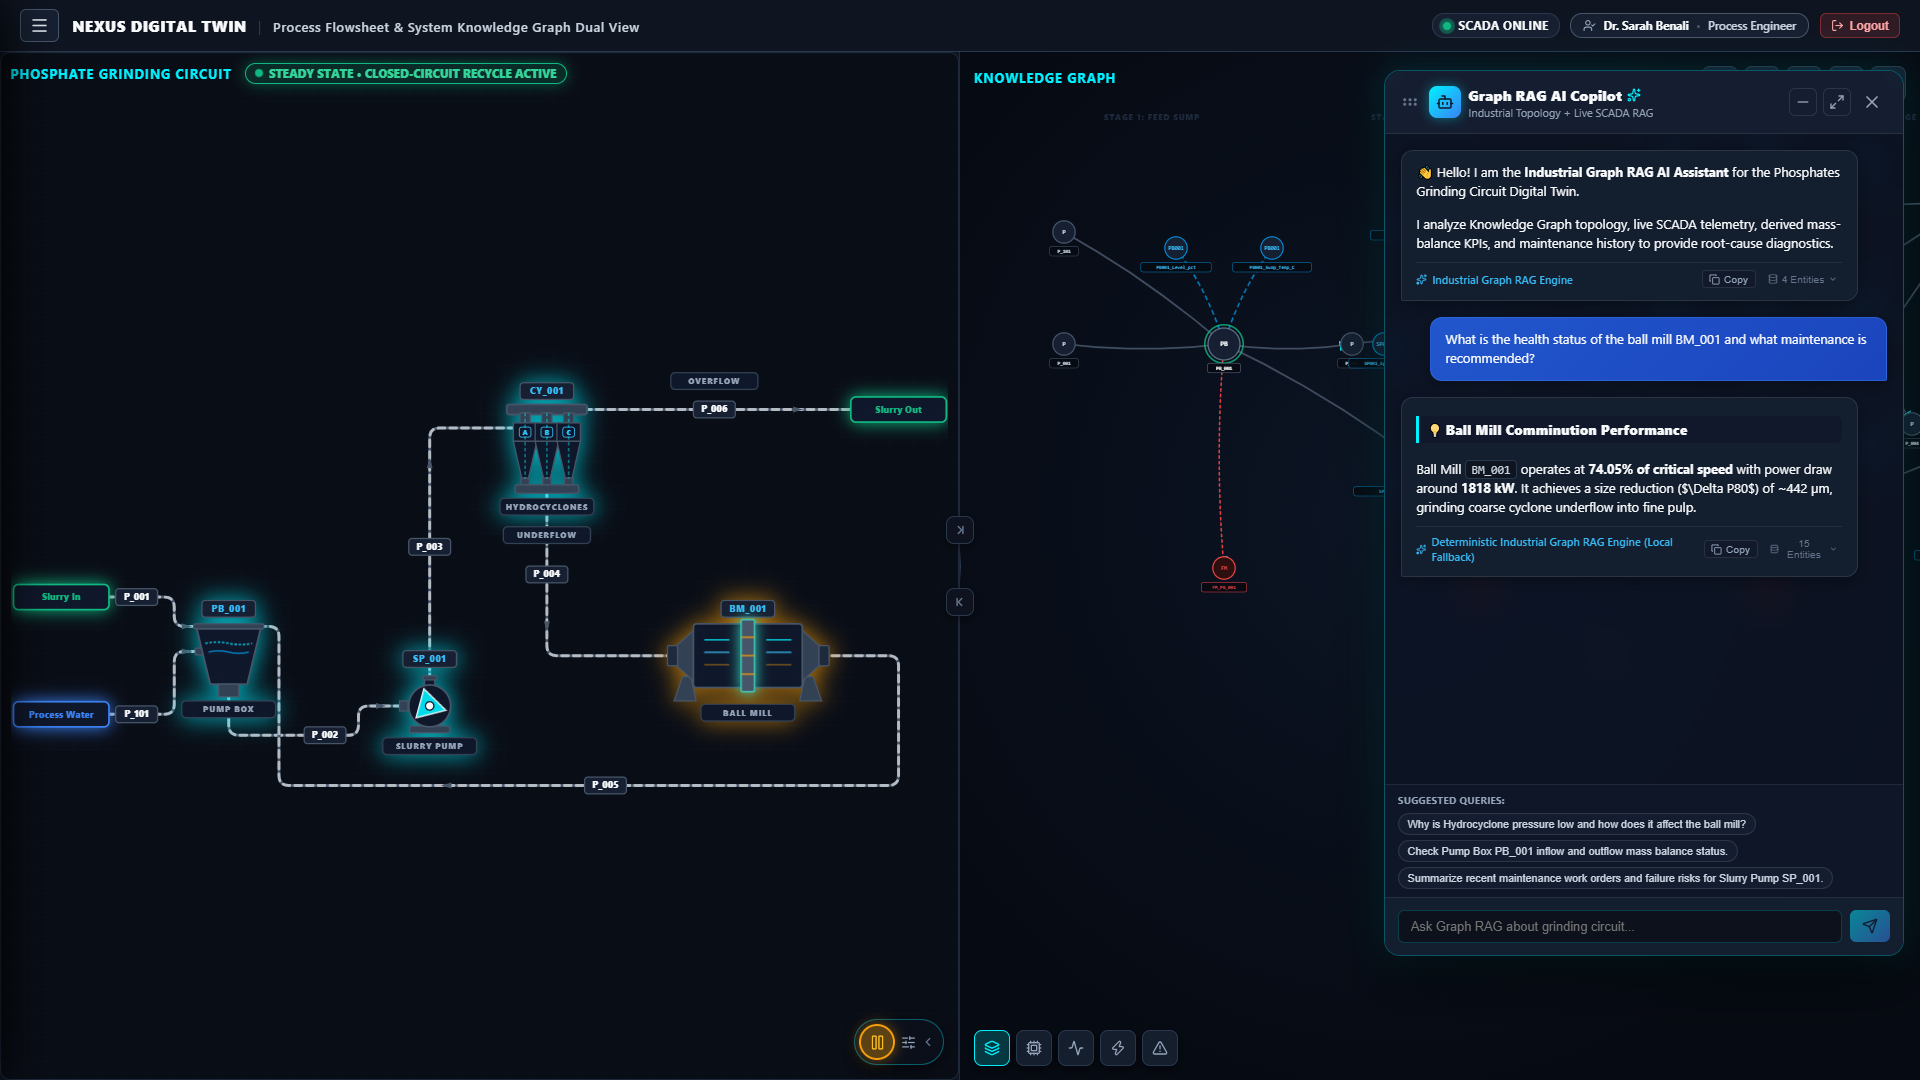
\includegraphics[width=\textwidth]{app_copilot}
\caption{Copilote Graph RAG : réponse sur l'état du broyeur BM\_001}
\label{fig:copilot}
\end{figure}

\section{Évaluation}

\subsection{Capteur virtuel du P80 par XGBoost}
\label{sec:xgboost}

\paragraph{Objectif.} Estimer en continu le P80 de la surverse des hydrocyclones, c'est-à-dire la finesse du produit envoyé en aval, sans attendre une analyse granulométrique.

\paragraph{Données.} Le modèle est entraîné sur les données du jumeau (dossier \texttt{data/}) : 2\,880 mesures procédé acquises toutes les 15 minutes du 1\textsuperscript{er} au 30 juillet 2026, et 43\,200 mesures de santé acquises chaque minute. Chaque mesure procédé est associée à la \textbf{moyenne des signaux de santé sur les 15 minutes qui la précèdent}, ce qui reprend le principe d'alignement temporel décrit à la section~\ref{sec:asymetrie}. Sur cette période, le P80 de la surverse varie entre 135,7 et 149,9~µm (moyenne 142,7~µm, écart-type 3,67~µm).

\paragraph{Choix des variables et prévention des fuites.} Un capteur virtuel ne doit utiliser que des grandeurs réellement disponibles au moment de l'estimation. Toutes les granulométries et teneurs mesurées en aval, ainsi que le rapport de réduction (calculé à partir du P80), ont donc été \textbf{exclues}, car elles contiennent la réponse. Deux scénarios ont été évalués :
\begin{itemize}
  \item \textbf{Scénario A -- capteurs en ligne} (32 variables) : débits et fractions solides des différentes lignes (débitmètres et densimètres), ainsi que les signaux de santé des équipements (puissance et vitesse du broyeur, pressions des cyclones, vitesse de la pompe, niveau du bac, etc.) ;
  \item \textbf{Scénario B -- A + caractérisation de l'alimentation} (34 variables) : on ajoute le P80 et la teneur BPL de l'alimentation fraîche, connus en amont du circuit.
\end{itemize}

\paragraph{Protocole.} Pour respecter la nature temporelle des données, le découpage est \textbf{chronologique} : 70\,\% pour l'entraînement (2\,015 points), 15\,\% pour la validation (433 points) et 15\,\% pour le test (432 points, du 26 au 30 juillet). Un découpage aléatoire aurait laissé le modèle «~voir le futur~» et surestimé ses performances. Les hyperparamètres de XGBoost~\cite{chen2016} (profondeur, taux d'apprentissage, sous-échantillonnage) sont choisis par recherche de grille, avec arrêt anticipé sur le jeu de validation. Le modèle final est ensuite réentraîné sur l'entraînement et la validation, puis évalué une seule fois sur le test. Trois modèles servent de comparaison :
\begin{itemize}
  \item une prédiction constante égale à la moyenne, qui sert de plancher ;
  \item une régression linéaire régularisée (Ridge) ;
  \item un Random Forest avec les mêmes hyperparamètres que le simulateur What-If du backend.
\end{itemize}
Les performances sont mesurées par le coefficient de détermination $R^2$, la \gls{rmse}, la \gls{mae} et l'erreur relative moyenne (MAPE) :
\[
\mathrm{RMSE}=\sqrt{\frac{1}{n}\sum_{i=1}^{n}(y_i-\hat{y}_i)^2}, \qquad
\mathrm{MAE}=\frac{1}{n}\sum_{i=1}^{n}\lvert y_i-\hat{y}_i\rvert, \qquad
R^2 = 1-\frac{\sum_i (y_i-\hat{y}_i)^2}{\sum_i (y_i-\bar{y})^2}
\]

\paragraph{Résultats.} Le tableau~\ref{tab:resp80} et la figure~\ref{fig:r2comp} présentent les performances sur le jeu de test.

\begin{table}[H]
\centering
\caption{Performance des modèles sur le jeu de test (432 points, 26--30 juillet 2026)}
\label{tab:resp80}
\small\setlength{\tabcolsep}{5pt}
\begin{tabular}{llcccc}
\toprule
\textbf{Scénario} & \textbf{Modèle} & $\boldsymbol{R^2}$ & \textbf{RMSE (µm)} & \textbf{MAE (µm)} & \textbf{MAPE} \\
\midrule
\multirow{4}{*}{A -- en ligne}
 & Moyenne (référence) & $-0{,}025$ & 3,916 & 3,542 & 2,50\,\% \\
 & Régression Ridge & 0,890 & 1,281 & 1,002 & 0,70\,\% \\
 & Random Forest & 0,953 & 0,842 & 0,672 & 0,47\,\% \\
 & \textbf{XGBoost} & \textbf{0,950} & \textbf{0,869} & \textbf{0,669} & \textbf{0,47\,\%} \\
\midrule
\multirow{4}{*}{B -- + alimentation}
 & Moyenne (référence) & $-0{,}025$ & 3,916 & 3,542 & 2,50\,\% \\
 & Régression Ridge & 0,950 & 0,861 & 0,662 & 0,47\,\% \\
 & Random Forest & 0,952 & 0,845 & 0,667 & 0,47\,\% \\
 & \textbf{XGBoost} & \textbf{0,953} & \textbf{0,841} & \textbf{0,657} & \textbf{0,46\,\%} \\
\bottomrule
\end{tabular}
\end{table}

\begin{figure}[H]
\centering
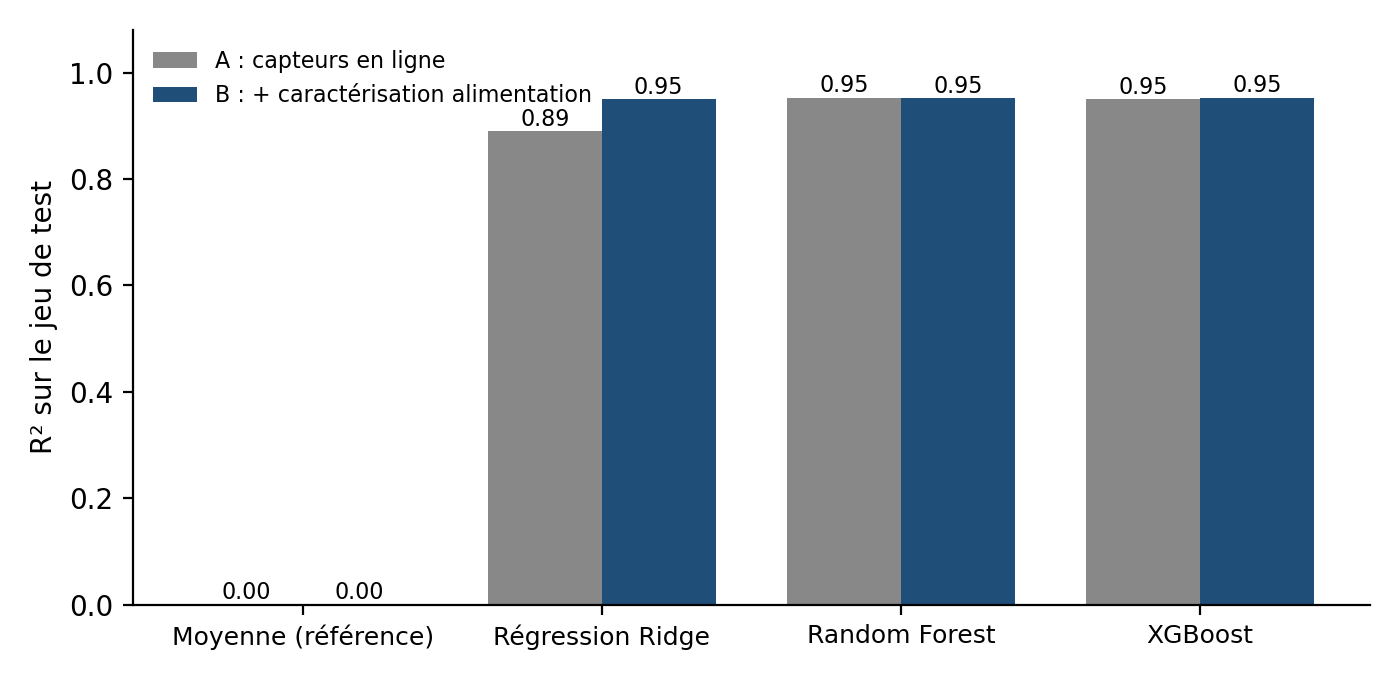
\includegraphics[width=0.85\textwidth]{models_r2_comparison}
\caption{Coefficient de détermination $R^2$ des quatre modèles sur le jeu de test, pour les deux scénarios}
\label{fig:r2comp}
\end{figure}

La figure~\ref{fig:p80ts} superpose le P80 mesuré et le P80 estimé par XGBoost sur toute la période de test, et la figure~\ref{fig:parity} compare les valeurs point par point.

\begin{figure}[H]
\centering
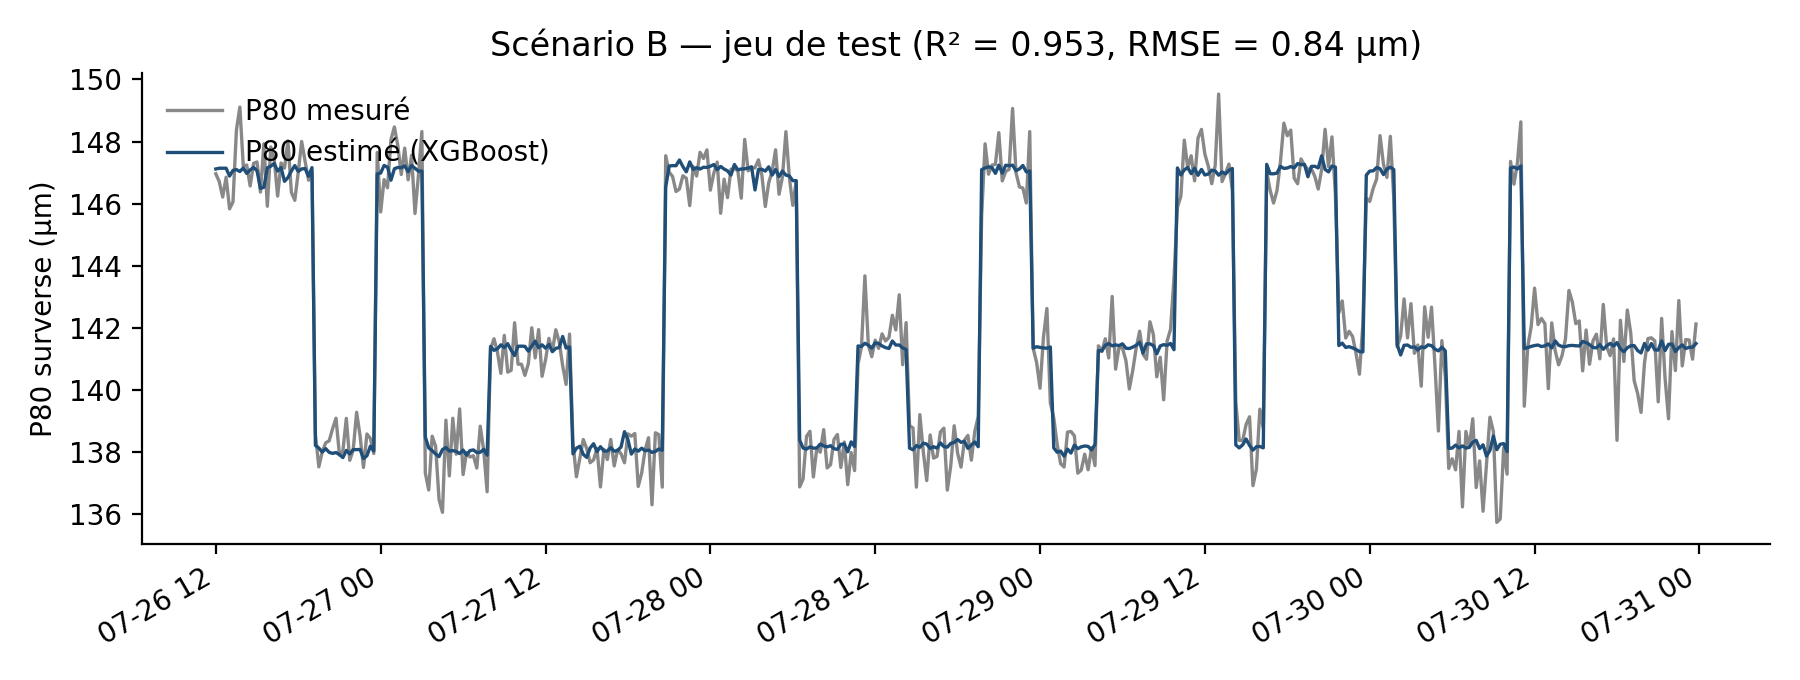
\includegraphics[width=\textwidth]{p80_timeseries_B}
\caption{P80 mesuré et P80 estimé par XGBoost sur le jeu de test (scénario B)}
\label{fig:p80ts}
\end{figure}

\begin{figure}[H]
\centering
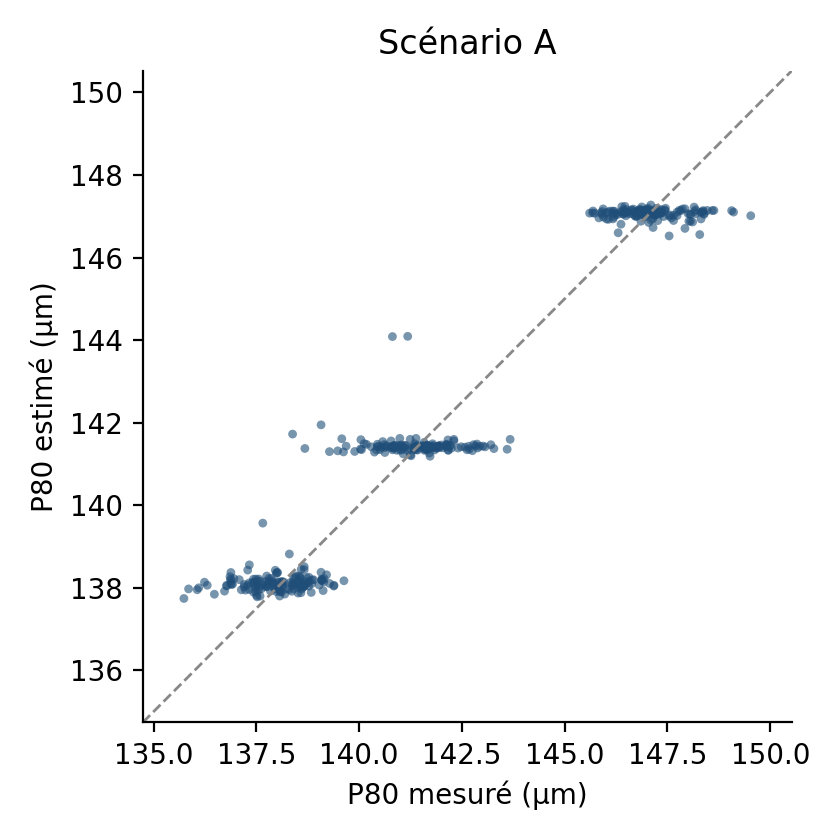
\includegraphics[width=0.45\textwidth]{p80_parity_A}\hfill
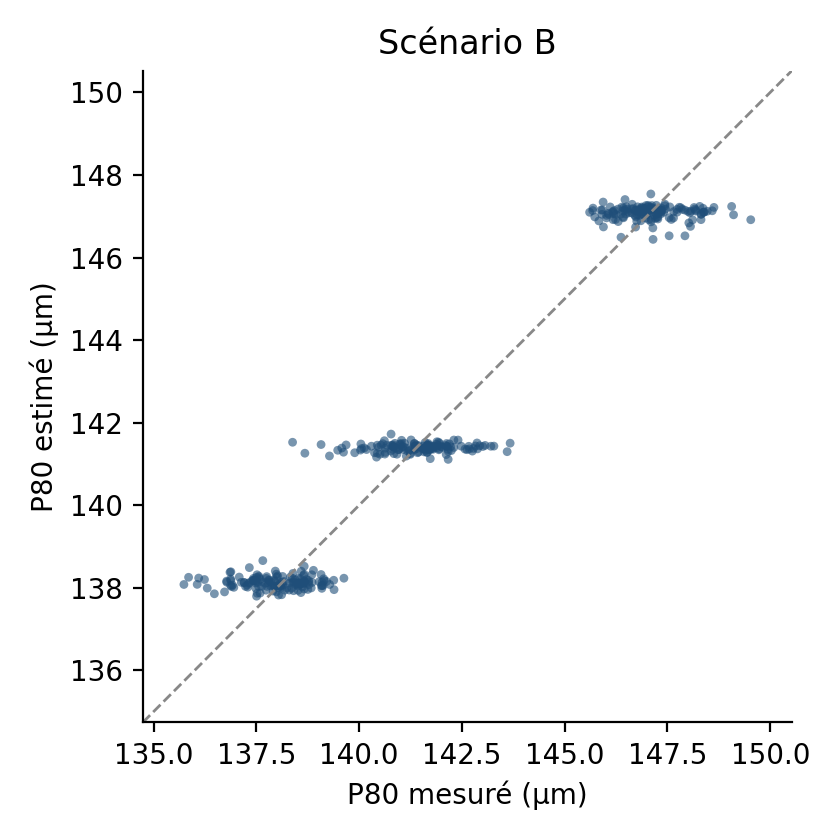
\includegraphics[width=0.45\textwidth]{p80_parity_B}
\caption{P80 estimé en fonction du P80 mesuré (la diagonale correspond à une estimation parfaite)}
\label{fig:parity}
\end{figure}

\paragraph{Robustesse.} Un seul découpage peut être favorable par hasard. Une validation croisée temporelle en 5 plis (\textit{TimeSeriesSplit}), où chaque pli teste le modèle sur une période postérieure à celle d'entraînement, donne pour XGBoost :
\begin{itemize}
  \item scénario A : $R^2 = 0{,}938 \pm 0{,}008$ et RMSE $= 0{,}93 \pm 0{,}06$~µm ;
  \item scénario B : $R^2 = 0{,}944 \pm 0{,}007$ et RMSE $= 0{,}88 \pm 0{,}03$~µm.
\end{itemize}
La faible dispersion d'un pli à l'autre montre que le modèle reste stable dans le temps.

\paragraph{Variables les plus influentes.} La figure~\ref{fig:importance} montre que, dans le scénario B, le modèle s'appuie d'abord sur la caractérisation de l'alimentation : P80 d'alimentation (55\,\% du gain total), teneur BPL (21\,\%) et débit solide d'alimentation (13\,\%). Dans le scénario A, en l'absence de ces analyses, il reconstitue l'information à partir des mesures hydrauliques : fraction solide de la surverse (36\,\%), débit de décharge du broyeur (23\,\%), débit de surverse (16\,\%) et débit d'alimentation (15\,\%). Ce comportement est cohérent avec la physique de la classification : la densité et le débit de la surverse dépendent directement de la coupure granulométrique des hydrocyclones~\cite{wills2016}.

\begin{figure}[H]
\centering
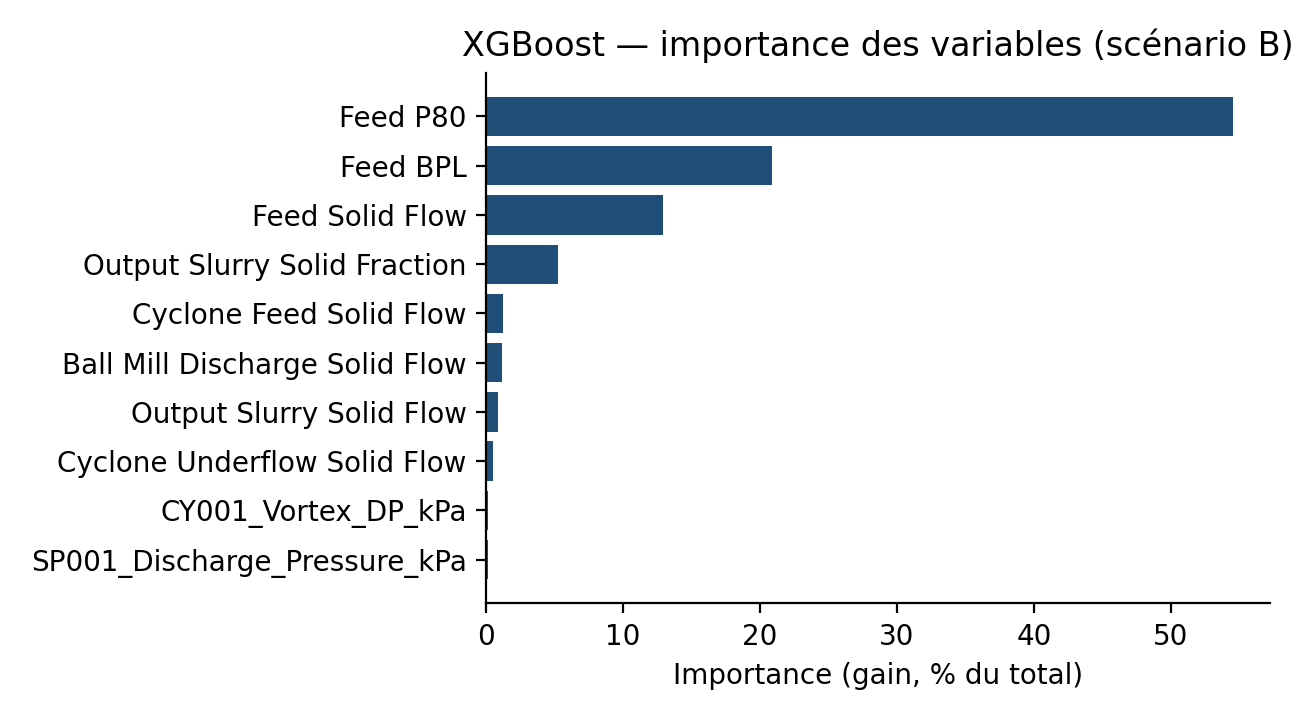
\includegraphics[width=0.75\textwidth]{xgb_feature_importance}
\caption{Importance des variables du modèle XGBoost (scénario B, gain normalisé)}
\label{fig:importance}
\end{figure}

\paragraph{Analyse.} Quatre enseignements se dégagent.
\begin{enumerate}
  \item \textbf{Le capteur virtuel est fiable.} Avec une erreur moyenne de 0,66~µm, soit 0,46\,\% du P80, XGBoost réduit l'erreur de 81\,\% par rapport à la référence constante (MAE de 3,54~µm).
  \item \textbf{Les capteurs en ligne suffisent.} Sans aucune analyse de laboratoire (scénario A), XGBoost atteint déjà $R^2 = 0{,}950$. Un modèle linéaire plafonne à 0,890 dans ce scénario : la relation entre les débits et la granulométrie n'est pas linéaire, ce qui justifie un modèle à base d'arbres.
  \item \textbf{XGBoost et Random Forest sont à égalité en précision.} Les écarts, de l'ordre de 0,003 en $R^2$, ne sont pas significatifs. XGBoost se distingue par sa \textbf{sobriété} : son modèle final comporte 49 arbres de profondeur 3 et pèse \textbf{0,06~Mo}, contre 100 arbres de profondeur 22 et \textbf{8,3~Mo} pour le Random Forest, soit un modèle environ 130 fois plus léger. C'est un atout pour un déploiement embarqué, au plus près des machines.
  \item \textbf{Le plafond observé est celui du bruit de mesure.} Les figures~\ref{fig:p80ts} et~\ref{fig:parity} montrent que le P80 évolue selon trois régimes de fonctionnement (environ 138, 141,5 et 147~µm) et que le modèle identifie chaque changement de régime sans retard. L'erreur résiduelle correspond aux fluctuations à l'intérieur d'un régime, qui ne sont liées à aucune variable d'entrée. Aucun modèle ne peut les prédire, ce qui explique que les trois modèles non linéaires convergent vers la même RMSE, environ 0,84~µm.
\end{enumerate}

\paragraph{Reproductibilité.} L'ensemble de l'expérience tient dans un script unique du projet, \nolinkurl{ml/soft_sensor_p80/train_xgboost.py}, avec une graine aléatoire fixée. Le script produit le fichier \texttt{metrics.json}, les figures de cette section et le modèle entraîné (\nolinkurl{xgb_soft_sensor_p80.joblib}).



\subsection{Simulateur What-If}
Le tableau~\ref{tab:whatif} regroupe par famille les $R^2$ que le backend calcule pour chacune des 23 sorties du simulateur. Ces scores sont obtenus sur 20\,\% des données tirés au hasard.

\begin{table}[H]
\centering
\caption{Précision du simulateur What-If ($R^2$ par sortie, découpage aléatoire 80/20)}
\label{tab:whatif}
\begin{tabularx}{\textwidth}{>{\raggedright\arraybackslash}p{4.6cm} c X}
\toprule
\textbf{Famille de sorties} & \textbf{$R^2$} & \textbf{Détail} \\
\midrule
Débits, teneurs et P80 (cyclones, broyeur, surverse) & 0,90 -- 1,00 & 12 sorties ; P80 de décharge du broyeur : 0,902 \\
Indicateurs de circuit & 0,996 -- 1,000 & Charge circulante, rapport de réduction \\
Santé du broyeur & 0,66 -- 0,78 & Puissance 0,754 ; courant 0,743 ; paliers 0,764--0,779 ; vibration 0,661 \\
Santé de la pompe & 0,67 -- 0,68 & Puissance 0,666 ; pression de refoulement 0,684 \\
Pressions des cyclones & 0,58 -- 0,60 & Pression d'entrée 0,596 ; pression différentielle 0,579 \\
\midrule
\textbf{Ensemble (23 sorties)} & \textbf{0,874} & Médiane 0,996 ; 13 sorties au-dessus de 0,95 \\
\bottomrule
\end{tabularx}
\end{table}

\paragraph{Analyse critique.} Les signaux de santé et de pression sont prédits nettement moins bien que les grandeurs de procédé. Ils dépendent en effet de phénomènes que les 8 entrées ne décrivent pas : usure, bruit de mesure, dynamique propre des équipements. L'interface le signale avec un badge de fiabilité. À l'inverse, les $R^2$ proches de 1 obtenus sur les grandeurs de procédé sont \textbf{optimistes}. Le modèle est entraîné sur l'historique fusionné par jointure temporelle, où chaque mesure de procédé est répétée sur 15 lignes consécutives (section~\ref{sec:asymetrie}). Un découpage aléatoire place donc dans le jeu de test des lignes presque identiques à des lignes d'entraînement. Le capteur XGBoost de la section~\ref{sec:xgboost} évite ce biais grâce à un découpage chronologique et à une agrégation à 15 minutes. Appliquer ce même protocole au simulateur What-If est une amélioration directe, décrite dans les perspectives.

\subsection{Persistance des données}
L'historien a été vérifié par des tests automatisés qui simulent un arrêt complet (tableau~\ref{tab:histtests}). La suite de tests du backend (15 tests) passe entièrement.

\begin{table}[H]
\centering
\caption{Vérification de l'historien de télémétrie}
\label{tab:histtests}
\begin{tabularx}{\textwidth}{X c}
\toprule
\textbf{Scénario de test} & \textbf{Résultat} \\
\midrule
251 messages reçus, arrêt, puis redémarrage de l'historien : les 251 lignes sont retrouvées & Réussi \\
Après redémarrage, les 100 derniers messages de chaque tag sont restaurés en mémoire & Réussi \\
Démarrage de l'API, réception de 30 messages Node-RED, arrêt complet puis redémarrage : 30 lignes conservées, historique restauré & Réussi \\
Requête filtrée par tag et export CSV par l'API & Réussi \\
Valeur non numérique : conservée dans le message JSON, sans erreur & Réussi \\
\bottomrule
\end{tabularx}
\end{table}

\subsection{Vérification des besoins}
\begin{table}[H]
\centering
\caption{Couverture des besoins fonctionnels}
\label{tab:couverture}
\begin{tabular}{llc}
\toprule
\textbf{Réf.} & \textbf{Besoin} & \textbf{Statut} \\
\midrule
BF1 & Authentification et rôles & \textcolor{vert}{Réalisé} \\
BF2 & Acquisition (relecture + OPC UA/Node-RED) & \textcolor{vert}{Réalisé} \\
BF3 & Pilotage de la simulation & \textcolor{vert}{Réalisé} \\
BF4 & Synoptique et fiches équipements & \textcolor{vert}{Réalisé} \\
BF5 & Graphe de connaissances & \textcolor{vert}{Réalisé} \\
BF6 & Vue 3D & \textcolor{vert}{Réalisé} \\
BF7 & Maintenance et fiabilité & \textcolor{vert}{Réalisé} \\
BF8 & Simulateur What-If & \textcolor{vert}{Réalisé} \\
BF9 & Copilote IA & \textcolor{vert}{Réalisé} \\
BF10 & Historique persistant & \textcolor{vert}{Réalisé} \\
\bottomrule
\end{tabular}
\end{table}

\section{Limites}
\label{sec:limites}
Une évaluation honnête du prototype conduit à relever plusieurs limites :
\begin{itemize}
  \item \textbf{Données simulées.} Les deux sources proviennent de données simulées (qualité \texttt{SIM} dans les messages). Les performances des modèles devront être confirmées sur des mesures réelles, plus bruitées et plus lacunaires.
  \item \textbf{Évaluation optimiste du What-If.} Comme on l'a vu plus haut, son découpage aléatoire surestime la précision sur les grandeurs de procédé.
  \item \textbf{Capteur virtuel hors ligne.} Le modèle XGBoost est entraîné et évalué, mais il n'est pas encore branché sur le flux temps réel du backend.
  \item \textbf{Absence de boucle de retour automatique.} Au sens de Kritzinger \textit{et al.}~\cite{kritzinger2018}, le système est une ombre numérique : il n'agit pas sur le procédé.
  \item \textbf{Pas de modèle physique.} Les modèles sont orientés données. Ils n'extrapolent pas en dehors des régimes observés dans l'historique.
  \item \textbf{Dépendance à un service externe.} Le copilote privilégie une API de LLM hébergée, ce qui pose des questions de confidentialité en milieu industriel. Le moteur local de secours n'en atténue qu'en partie l'impact.
\end{itemize}

\section{Conclusion}
Le prototype couvre l'ensemble des besoins fonctionnels identifiés, de l'acquisition OPC UA jusqu'à l'aide à la décision. Le capteur virtuel atteint une précision de l'ordre du bruit de mesure, l'historique survit désormais aux redémarrages, et les limites relevées tracent directement la feuille de route présentée en conclusion.

\chapitresansnumero{Conclusion générale et perspectives}

Ce projet de fin d'année visait à concevoir, au sein de JESA, une preuve de concept de jumeau numérique pour un circuit de broyage de phosphate. Trois difficultés avaient été identifiées : une qualité produit connue trop tard, une maintenance réactive et une information dispersée.

La solution y répond par une architecture en cinq couches.
\begin{itemize}
  \item \textbf{Acquisition.} Une chaîne industrielle KEPServerEX -- Node-RED (OPC UA) et une relecture des historiques publient 45 signaux sur un broker MQTT commun.
  \item \textbf{Traitement et stockage.} Un backend FastAPI organisé en domaines fusionne des flux acquis à des rythmes différents, calcule les bilans de matière et enregistre toute la télémétrie dans un historien SQLite. L'historique survit ainsi à un arrêt du poste.
  \item \textbf{Information métier.} Un graphe de connaissances de 69 nœuds relie équipements, capteurs, lignes, modes de défaillance et interventions de maintenance.
  \item \textbf{Intelligence artificielle.} Le simulateur What-If anticipe l'effet d'un réglage sur 23 grandeurs aval, et le copilote Graph RAG répond en langage naturel, même hors connexion. Enfin, le capteur virtuel XGBoost estime le P80 avec un $R^2$ de 0,953 et une erreur moyenne de 0,66~µm, sur une période de test qu'il n'avait jamais vue.
\end{itemize}

Sur le plan personnel, ce stage m'a permis de confronter ma formation d'ingénieure à la réalité d'un procédé industriel, de l'automate jusqu'au tableau de bord. J'ai découvert que la valeur d'une donnée dépend autant de sa compréhension physique (ce que représente un P80, pourquoi un palier chauffe) que de la rigueur avec laquelle on l'évalue. Un découpage chronologique ou aléatoire peut à lui seul changer la conclusion que l'on tire d'un modèle.

\section*{Perspectives}
Les limites relevées à la section~\ref{sec:limites} dessinent la suite du travail :
\begin{itemize}
  \item \textbf{Capteur virtuel en temps réel.} Brancher le modèle XGBoost sur le flux MQTT et republier le P80 estimé comme un tag à part entière.
  \item \textbf{Évaluation rigoureuse du What-If.} Réentraîner le simulateur avec un découpage chronologique sur des données agrégées à 15 minutes, comme pour le capteur virtuel, afin d'obtenir une mesure non biaisée de sa précision.
  \item \textbf{Validation sur site réel.} Connecter Node-RED aux automates d'une installation OCP et entraîner les modèles sur l'historique réel accumulé par l'historien.
  \item \textbf{Surveillance des modèles.} Détecter la dérive du procédé (dureté du minerai, usure) et déclencher le réentraînement des modèles~\cite{kadlec2009}.
  \item \textbf{Détection d'anomalies.} Exploiter l'historique des signaux de santé pour détecter automatiquement les comportements anormaux du broyeur et de la pompe.
  \item \textbf{Vers un vrai jumeau.} Proposer des consignes validées par l'opérateur, puis, à terme, fermer la boucle de régulation~\cite{kritzinger2018}.
  \item \textbf{Modèles hybrides.} Coupler les modèles orientés données à des modèles physiques du broyage et de la classification~\cite{wills2016}.
\end{itemize}


\cleardoublepage
\phantomsection
\addcontentsline{toc}{chapter}{Bibliographie}
\markboth{Bibliographie}{Bibliographie}
\begin{thebibliography}{99}
\small

% ------------------------------------------------ Contexte : JESA, OCP, phosphate
\bibitem{jesaabout} JESA Group, «~About us~», \url{https://www.jesagroup.com/about.html}, consulté en septembre 2026.

\bibitem{jesawiki} «~JESA Group~», \textit{Wikipédia}, \url{https://fr.wikipedia.org/wiki/JESA_Group}, consulté en septembre 2026.

\bibitem{jacobsteammaroc} Jacobs Engineering Group, «~Jacobs Engineering SA Announces Acquisition of Team Maroc~», communiqué de presse, 22 juin 2012, \url{https://www.jacobs.com/newsroom/press-release/jacobs-engineering-sa-announces-acquisition-team-maroc}.

\bibitem{worleyasx} WorleyParsons Limited, «~WorleyParsons completes acquisition of Jacobs ECR division~», annonce ASX, 29 avril 2019, \url{https://announcements.asx.com.au/asxpdf/20190429/pdf/444lf4cw4vp0mc.pdf}.

\bibitem{usgs2026} S.~M. Jasinski, «~Phosphate Rock~», in \textit{Mineral Commodity Summaries 2026}, U.S. Geological Survey, février 2026, \url{https://pubs.usgs.gov/periodicals/mcs2026/mcs2026-phosphate.pdf}.

\bibitem{ocpwiki} «~OCP Group~», \textit{Wikipedia}, \url{https://en.wikipedia.org/wiki/OCP_Group}, consulté en septembre 2026.

\bibitem{ocpresultats2025} «~OCP Group Reports 17\% Revenue Growth in 2025, Reaches MAD 114 Billion~», \textit{Morocco World News}, février 2026, \url{https://www.moroccoworldnews.com/2026/02/281063/ocp-group-reports-17-revenue-growth-in-2025-reaches-mad-114-billion/}.

\bibitem{ocppipeline} OCP Group, «~Commissioning of the Slurry Pipeline connecting Khouribga to Jorf Lasfar~», \url{https://www.ocpgroup.ma/en/commissioning-slurry-pipeline-connecting-khouribga-jorf-lasfar}, consulté en septembre 2026.

\bibitem{cooper1990} R.~G. Cooper, «~Stage-gate systems: a new tool for managing new products~», \textit{Business Horizons}, vol.~33, n\textsuperscript{o}~3, p.~44--54, 1990.

% ------------------------------------------------ Procédé
\bibitem{wills2016} B.~A. Wills et J.~A. Finch, \textit{Wills' Mineral Processing Technology}, 8\textsuperscript{e} éd., Butterworth-Heinemann, 2016.

\bibitem{jeswiet2016} J. Jeswiet et A. Szekeres, «~Energy Consumption in Mining Comminution~», \textit{Procedia CIRP}, vol.~48, p.~140--145, 2016.

% ------------------------------------------------ Jumeau numérique
\bibitem{grieves2017} M. Grieves et J. Vickers, «~Digital Twin: Mitigating Unpredictable, Undesirable Emergent Behavior in Complex Systems~», in \textit{Transdisciplinary Perspectives on Complex Systems}, Springer, p.~85--113, 2017.

\bibitem{glaessgen2012} E.~H. Glaessgen et D.~S. Stargel, «~The Digital Twin Paradigm for Future NASA and U.S. Air Force Vehicles~», \textit{53rd AIAA/ASME/ASCE/AHS/ASC Structures, Structural Dynamics and Materials Conference}, AIAA 2012-1818, 2012.

\bibitem{kritzinger2018} W. Kritzinger, M. Karner, G. Traar, J. Henjes et W. Sihn, «~Digital Twin in manufacturing: A categorical literature review and classification~», \textit{IFAC-PapersOnLine}, vol.~51, n\textsuperscript{o}~11, p.~1016--1022, 2018.

\bibitem{tao2018} F. Tao, M. Zhang, Y. Liu et A.~Y.~C. Nee, «~Digital twin driven prognostics and health management for complex equipment~», \textit{CIRP Annals}, vol.~67, n\textsuperscript{o}~1, p.~169--172, 2018.

\bibitem{tao2019} F. Tao, H. Zhang, A. Liu et A.~Y.~C. Nee, «~Digital Twin in Industry: State-of-the-Art~», \textit{IEEE Transactions on Industrial Informatics}, vol.~15, n\textsuperscript{o}~4, p.~2405--2415, 2019.

\bibitem{sethi2017} P. Sethi et S.~R. Sarangi, «~Internet of Things: Architectures, Protocols, and Applications~», \textit{Journal of Electrical and Computer Engineering}, vol.~2017, article 9324035, 2017.

\bibitem{ibmdt} IBM, «~What is a digital twin?~», \url{https://www.ibm.com/think/topics/digital-twin}, consulté en septembre 2026.

\bibitem{dtccpt} Digital Twin Consortium, \textit{Digital Twin Capabilities Periodic Table -- User Guide}, 2022, \url{https://www.digitaltwinconsortium.org/initiatives/capabilities-periodic-table/}.

\bibitem{doeom} G.~P. Sullivan, R. Pugh, A.~P. Melendez et W.~D. Hunt, \textit{Operations \& Maintenance Best Practices -- A Guide to Achieving Operational Efficiency}, Release 3.0, U.S. Department of Energy, Federal Energy Management Program, 2010.

% ------------------------------------------------ IA
\bibitem{breiman2001} L. Breiman, «~Random Forests~», \textit{Machine Learning}, vol.~45, n\textsuperscript{o}~1, p.~5--32, 2001.

\bibitem{kadlec2009} P. Kadlec, B. Gabrys et S. Strandt, «~Data-driven Soft Sensors in the process industry~», \textit{Computers \& Chemical Engineering}, vol.~33, n\textsuperscript{o}~4, p.~795--814, 2009.

\bibitem{chen2016} T. Chen et C. Guestrin, «~XGBoost: A Scalable Tree Boosting System~», \textit{Proceedings of the 22nd ACM SIGKDD International Conference on Knowledge Discovery and Data Mining}, p.~785--794, 2016.


\bibitem{lewis2020} P. Lewis \textit{et al.}, «~Retrieval-Augmented Generation for Knowledge-Intensive NLP Tasks~», \textit{Advances in Neural Information Processing Systems (NeurIPS)}, vol.~33, 2020.

\bibitem{edge2024} D. Edge \textit{et al.}, «~From Local to Global: A Graph RAG Approach to Query-Focused Summarization~», arXiv:2404.16130, 2024.

\bibitem{sklearn} F. Pedregosa \textit{et al.}, «~Scikit-learn: Machine Learning in Python~», \textit{Journal of Machine Learning Research}, vol.~12, p.~2825--2830, 2011.


% ------------------------------------------------ Normes et protocoles
\bibitem{isa101} ANSI/ISA-101.01-2015, \textit{Human Machine Interfaces for Process Automation Systems}, International Society of Automation, 2015.

\bibitem{iec62541} IEC 62541, \textit{OPC Unified Architecture}, International Electrotechnical Commission (série de normes).

\bibitem{mqtt5} OASIS, \textit{MQTT Version 5.0}, OASIS Standard, 7 mars 2019, \url{https://docs.oasis-open.org/mqtt/mqtt/v5.0/mqtt-v5.0.html}.

% ------------------------------------------------ Outils
\bibitem{merkel2014} D. Merkel, «~Docker: lightweight Linux containers for consistent development and deployment~», \textit{Linux Journal}, n\textsuperscript{o}~239, 2014.

\bibitem{kepware} PTC, «~KEPServerEX~», documentation, \url{https://www.ptc.com/en/products/kepware/kepserverex}.

\bibitem{nodered} OpenJS Foundation, «~Node-RED: Low-code programming for event-driven applications~», \url{https://nodered.org/docs/}.


\bibitem{fastapi} S. Ramírez, «~FastAPI~», documentation, \url{https://fastapi.tiangolo.com/}.


\bibitem{sqlite} SQLite Consortium, «~SQLite Documentation -- Write-Ahead Logging~», \url{https://www.sqlite.org/wal.html}.

\bibitem{neo4j} Neo4j, Inc., «~Neo4j Graph Database Documentation~», \url{https://neo4j.com/docs/}.


\bibitem{react} Meta Open Source, «~React~», documentation, \url{https://react.dev/}.

\bibitem{r3f} Poimandres, «~React Three Fiber~», documentation, \url{https://r3f.docs.pmnd.rs/}.

\end{thebibliography}


\end{document}
